\chapter{再生核Hilbert空间}
\label{chap:rkhs}

在区间上的几个位置测得一个量的数值，想由这些读数恢复整条函数，这是函数逼近最常见的入口。读数只有有限个，通过这些点的函数却有无穷多条；即使选定了一条，它在测点之间的误差也不受读数本身约束。要让这个问题可以讨论，候选函数所在的空间至少要让“在一点取值”既有确定意义，又随函数连续变化：两个在范数下接近的候选函数，读数也应当接近。

本章研究满足这一要求的Hilbert函数空间。第~\ref{sec:rkhs-recovery}节先在有限特征空间中提出精确插值、带残差拟合与域外误差三个问题，并说明为什么点值必须受范数控制。第~\ref{sec:rkhs-reproducing-relation}节把每个点评估都连续的空间称为再生核Hilbert空间，用Riesz表示把读数写成与一个固定函数的内积，由此得到再生核。第~\ref{sec:rkhs-from-kernel}节反过来只从正定核出发构造空间，第~\ref{sec:rkhs-kernel-constructions}节给出由特征、非负组合和逐点乘积得到新核的规则。

有了核以后，有限观测问题可以完整地写成Gram矩阵的语言。第~\ref{sec:rkhs-min-norm-interpolation}节用观测映射与观测零空间的正交分解判断数据能否被插值，并求出唯一的最小范数插值函数。第~\ref{sec:rkhs-finite-subspaces}节转向表示误差：在已知函数的前提下，用核截面或一般有限特征张成的子空间去逼近它。第~\ref{sec:rkhs-mercer}节再加入参考测度，用核积分算子的谱得到Mercer展开和RKHS中的谱坐标，并比较截断误差在两种范数下的差别。

本章所用的Hilbert空间、正交投影、Riesz表示和紧自伴算子的谱定理分别来自第~\ref{chap:inner-product-spaces}章、第~\ref{chap:linear-functionals}章和第~\ref{chap:operator-spectra}章，完备化与零距离商来自第~\ref{chap:metric-spaces}章。读数带噪声时怎样选择损失与正则项、怎样求解相应的拟合问题，属于卷五的函数拟合；观测位置随机抽取时的统计误差属于卷八。本章只建立这些问题共同使用的空间结构与有限表示。

\section{从离散观测恢复函数}
\label{sec:rkhs-recovery}

设在位置$x_1,\ldots,x_n$处读到数值$y_1,\ldots,y_n$，我们想找一个函数$f$，使$f(x_i)$与$y_i$相符。先看一个最小的例子：在$[0,1]$上取$x=0,\tfrac12,1$，读数为$y=(0,1,0)$。抛物线$q(x)=4x(1-x)$与正弦曲线$s(x)=\sin(\pi x)$都恰好通过这三个点，把$q$加上任意倍数的$x(x-\tfrac12)(x-1)$也是如此。

这些函数在测点上完全一致，在测点之间却各不相同。例如在$x=\tfrac14$处，$q(\tfrac14)=0.75$，$s(\tfrac14)=\tfrac{\sqrt2}{2}\approx0.707$，而$x(x-\tfrac12)(x-1)$在该点等于$\tfrac{3}{64}$，乘上不同的系数可以得到任意的取值。所以有限个点值通常不能唯一确定整条函数，必须先说明在哪一类函数中寻找。

即使限定了候选函数的范围，仍有三个不同的问题。第一是\emph{精确插值}：是否存在候选函数在每个测点上都等于读数，若存在，怎样在众多可行函数中选出一个。第二是\emph{带残差的拟合}：读数含有误差时，强求精确通过反而会把误差写进函数，这时允许$f(x_i)$与$y_i$有偏差，再权衡偏差与函数本身的复杂程度。第三是\emph{域外误差}：所选函数与真实函数在测点之外相差多少，这已经不是读数本身能回答的问题。

本章主要处理第一个问题及第三个问题中只依赖空间结构的部分。第二个问题需要选择损失与正则项，归卷五的函数拟合。当测点由随机抽样产生时，域外误差还涉及样本量与置信水平，即统计意义上的泛化保证，可参考\BookChapterRef{chap:finite-sample-error-bounds}{卷八第4章“有限样本的误差上界”}；本章不讨论随机性。

\subsection{有限特征空间}
\label{sec:rkhs-finite-feature-space}

最直接的做法是预先固定有限个函数$\phi_1,\ldots,\phi_d$，只在它们的线性组合中寻找候选函数：
\[
f_{\bm\theta}(x)=\sum_{k=1}^d\theta_k\phi_k(x),\qquad \bm\theta\in\mathbb R^d .
\]
这些$\phi_k$称为特征或基函数。这样，寻找函数就变成寻找有限个系数，观测条件也随之变成线性方程。

把第$i$个测点处各特征的取值排成一行，得到$n\times d$的\term{设计矩阵}（design matrix）$\bm A$，其元素为$\bm A_{i,k}=\phi_k(x_i)$。于是$f_{\bm\theta}$在全部测点上的取值向量就是$\bm A\bm\theta$，精确插值的条件是
\begin{equation}
\bm A\bm\theta=\bm y .
\label{eq:rkhs-design-equation}
\end{equation}
这是卷二讨论过的线性方程：方程相容当且仅当$\bm y$属于$\bm A$的列空间；相容时，解唯一当且仅当$\bm A$的列线性无关，即$\operatorname{rank}\bm A=d$；不相容时，可以改求使$\lVert\bm A\bm\theta-\bm y\rVert_2$最小的最小二乘解，解不唯一时再从中选出欧氏长度最小的一个。这些判据与选解方法可参考\BookChapterRef{chap:linear-solution-selection}{卷二第9章“线性方程与最小二乘的选解”}。

\begin{example}[多项式特征下的三种情形]
\label{ex:rkhs-polynomial-features}
仍取测点$0,\tfrac12,1$与读数$\bm y=(0,1,0)^{\top}$，依次增加多项式特征的个数。
\begin{enumerate}
\item 取$\phi_1=1,\phi_2=x$。设计矩阵的三行是$(1,0)$、$(1,\tfrac12)$、$(1,1)$，秩为$2$。三个点不共线，$\bm y$不在列空间中，方程无解；最小二乘给出常数$\tfrac13$，残差不为零。
\item 再加入$\phi_3=x^2$。设计矩阵是$3\times3$的Vandermonde矩阵，测点互异，矩阵可逆，唯一解对应$q(x)=4x-4x^2$。
\item 再加入$\phi_4=x^3$。矩阵为$3\times4$，秩仍为$3$，零空间是一维的。$x(x-\tfrac12)(x-1)=x^3-\tfrac32x^2+\tfrac12x$在三个测点上为零，所以$q+t\,x(x-\tfrac12)(x-1)$对任意实数$t$都是精确插值。
\end{enumerate}
\end{example}

这个例子说明，表示维数改变的不只是方程的形状，还有候选函数本身。维数太低时数据可能无法实现；维数恰好时插值唯一；维数再增加，测点就不足以区分全部候选函数。可见“解是否存在、是否唯一”是候选空间与测点共同决定的性质，不是读数单独决定的。

更重要的是，观测残差为零并不保证整个定义域上的误差为零。若真实函数是$s(x)=\sin(\pi x)$，第2种情形得到的$q$在三个测点上与$s$完全一致，在$x=\tfrac14$处却相差约$0.043$。在第3种情形中，误差还会随$t$的选择任意变化。要谈论测点之外的误差，必须对候选函数加上读数之外的约束。

\subsection{点值观测的稳定性}
\label{sec:rkhs-point-stability}

有限特征空间的做法依赖于事先选好的维数。另一种思路是让候选函数在一个无限维Hilbert空间$H$中变化，再用范数$\lVert f\rVert_H$衡量函数的大小，从可行函数中选范数最小者。这样做之前，需要先检查点值读数与这个范数是否相容。

我们希望的是：两个候选函数在范数下接近时，它们在每个测点上的读数也接近。写成不等式，就是对每个$x$存在常数$C_x$，使
\begin{equation}
\lvert f(x)-g(x)\rvert\leq C_x\lVert f-g\rVert_H\qquad(f,g\in H).
\label{eq:rkhs-stability-requirement}
\end{equation}
若这一点不成立，范数很小的函数仍可能在测点上有很大的读数，“选范数最小的可行函数”就失去了控制读数的意义。

\paragraph{$L^2$空间中点值的两个缺陷}

$L^2(0,1)$是最熟悉的函数Hilbert空间，但它不满足这个要求，而且失败的方式有两种。第一，$L^2$的元素是几乎处处相等的函数类。零函数与只在$x=\tfrac12$处取$1$的函数属于同一个元素，却给出不同的点值，所以“取$\tfrac12$处的值”在$L^2$上根本没有确定意义。

第二，即使只看连续函数，点值也不受$L^2$范数控制。尖峰函数$f_k(t)=\max(1-kt,0)$满足$f_k(0)=1$，而
\[
\lVert f_k\rVert_{L^2}^2=\int_0^{1/k}(1-kt)^2\,\mathrm dt=\frac{1}{3k},
\]
比值$f_k(0)/\lVert f_k\rVert_{L^2}=\sqrt{3k}$随$k$无界。也就是说，在$L^2$范数下任意小的扰动，可以把原点的读数改变$1$。

\paragraph{Sobolev空间中的点值}

把导数也计入范数，情况就不同了。第~\ref{chap:sobolev-spaces}章说明，一维Sobolev空间$H^1(0,1)$中的每个元素都有唯一的绝对连续代表，其几乎处处导数就是弱导数$f'\in L^2(0,1)$。以下总取这个代表，于是$f(x)$有确定的值，第一个缺陷消失。

对第二个缺陷，取任意$x,y\in[0,1]$，由绝对连续性有$f(x)=f(y)+\int_y^xf'(t)\,\mathrm dt$。对$y$在$[0,1]$上积分，得到
\[
f(x)=\int_0^1f(y)\,\mathrm dy+\int_0^1\!\!\int_y^xf'(t)\,\mathrm dt\,\mathrm dy ,
\]
第二项的绝对值不超过$\int_0^1\lvert f'\rvert$。再用Cauchy--Schwarz不等式把两个$L^1$范数换成$L^2$范数，得
\begin{equation}
\lvert f(x)\rvert\leq\lVert f\rVert_{L^2}+\lVert f'\rVert_{L^2}\leq\sqrt2\,\lVert f\rVert_{H^1},\qquad
\lVert f\rVert_{H^1}^2=\lVert f\rVert_{L^2}^2+\lVert f'\rVert_{L^2}^2 .
\label{eq:rkhs-h1-point-bound}
\end{equation}
这正是要求~\eqref{eq:rkhs-stability-requirement}，而且常数$\sqrt2$对所有$x$通用。尖峰$f_k$在这里不再是反例：它的导数在$[0,1/k]$上等于$-k$，$\lVert f_k'\rVert_{L^2}^2=k$，$H^1$范数随$k$增大。

\paragraph{候选空间与真实函数}

所以候选空间必须同时满足两项要求：元素是在每一点都有确定取值的函数，并且每个点的读取都受范数控制。前者由空间的选取保证，后者取决于空间所带的范数；$L^2$两项都不满足，$H^1(0,1)$两项都满足。

需要注意的是，这两项要求只针对候选函数，并不断言真实函数属于该空间。若真实的量在$x=\tfrac12$处有跳跃，它就不属于$H^1(0,1)$，在$H^1$中寻找插值函数仍然可行，但得到的只是一个连续的替代品，跳跃附近的误差不会因为读数增多而自动消失。候选空间是否贴合真实函数，要结合问题本身判断，不由点值的稳定性推出。下一节把满足这两项要求的空间抽象出来。

\section{再生关系}
\label{sec:rkhs-reproducing-relation}

上一节得到候选空间的两项要求：元素是真正的函数，每个点的读取随函数连续变化。把这两项要求作为定义，就得到本章的空间。

全章的数域记为$\mathbb K$，取$\mathbb R$或$\mathbb C$。复内积沿用全书的约定：$\langle f,g\rangle$对第一个变量共轭线性、对第二个变量线性。主线中的例子都是实值函数，此时共轭不起作用；保留复数情形，是为了第~\ref{sec:rkhs-mercer}节使用复Hilbert空间上的谱定理时不必另行改写。

\begin{definition}[再生核Hilbert空间]
\label{def:rkhs-rkhs}
设$X$是非空集合，$H$是由函数$f:X\to\mathbb K$组成的Hilbert空间，其加法与数乘按逐点方式定义。对$x\in X$，称$\delta_x:H\to\mathbb K$，$\delta_x(f)=f(x)$为$x$处的\term{点评估泛函}（evaluation functional）。若对每个$x\in X$，$\delta_x$都是有界线性泛函，则称$H$为$X$上的\term{再生核Hilbert空间}（reproducing kernel Hilbert space），简称RKHS。
\end{definition}

定义中有两个条件。逐点运算这一条保证$H$的零元就是处处为零的函数，因而“两个元素相等”与“两个函数在每一点取值相同”是同一件事；$L^2$的元素是函数类，不在这个定义的讨论范围内。

有界性一条就是上一节的要求~\eqref{eq:rkhs-stability-requirement}：$\delta_x$线性且有界，等价于存在$C_x$使$\lvert f(x)\rvert\leq C_x\lVert f\rVert_H$，把$f$换成$f-g$就得到要求的不等式。定义只要求每个点各有一个常数$C_x$，不要求这些常数有共同上界。是否存在统一的常数，下文会由核在对角线上的取值读出。

\subsection{点评估界}
\label{sec:rkhs-evaluation-bounds}

判断一个函数空间是不是RKHS，关键是对每个$x$估计$\lvert f(x)\rvert/\lVert f\rVert_H$。先看有限维空间，再看一个无限维空间。

\paragraph{仿射函数空间}

设$X=\mathbb R$，令$H_{\mathrm{aff}}$为仿射函数$f(t)=a+bt$全体，内积取系数向量的内积：
\[
\langle a+bt,\ a'+b't\rangle=\overline a\,a'+\overline b\,b' .
\]
系数$(a,b)$与函数一一对应，所以$H_{\mathrm{aff}}$与$\mathbb K^2$等距同构，是二维Hilbert空间。

对固定的$x$，函数值是系数向量$(a,b)$与$(1,x)$的内积，由Cauchy--Schwarz不等式，
\[
\lvert f(x)\rvert=\lvert a\cdot1+b\cdot x\rvert\leq\sqrt{1+x^2}\,\lVert f\rVert .
\]
因此每个点评估都有界，$H_{\mathrm{aff}}$是RKHS。常数$\sqrt{1+x^2}$随$\lvert x\rvert$增大而无界，在整条实轴上没有统一的常数；若把定义域限制为$[-1,1]$，统一常数是$\sqrt2$。

同样的计算适用于次数不超过$m$的多项式空间，只是常数变为$(\sum_{k\leq m}\lvert x\rvert^{2k})^{1/2}$。更一般地，任何有限维函数空间配上任何内积都是RKHS，因为有限维赋范空间上的线性泛函都有界。点评估界真正需要论证的是无限维的情形。

\paragraph{左端固定的一阶Sobolev函数}

取$X=[0,1]$，令$H_{\min}$为$H^1(0,1)$中满足$f(0)=0$的实值函数全体，每个元素取其绝对连续代表，内积只用导数：
\[
\langle f,g\rangle_{H_{\min}}=\int_0^1f'(t)\,g'(t)\,\mathrm dt .
\]
先核对这是内积。若$\langle f,f\rangle=0$，则$f'=0$几乎处处，绝对连续性给出$f(x)=f(0)+\int_0^xf'=0$。这里由$f(0)=0$排除了常数函数，导数的$L^2$范数才能成为范数。

再核对完备性。映射$f\mapsto f'$把$H_{\min}$映到$L^2(0,1)$，保持内积。反过来，对任意$g\in L^2(0,1)$，函数$x\mapsto\int_0^xg$绝对连续，左端为零，导数几乎处处等于$g$，所以这个映射是满射。因此$H_{\min}$与$L^2(0,1)$等距同构，它继承了完备性，是无限维Hilbert空间。

点评估界来自同一个积分表示。对$x\in[0,1]$，把$f(x)$写成导数的累计，再用Cauchy--Schwarz不等式：
\begin{equation}
\lvert f(x)\rvert=\Bigl\lvert\int_0^xf'(t)\,\mathrm dt\Bigr\rvert
\leq\sqrt x\,\lVert f\rVert_{H_{\min}} .
\label{eq:rkhs-hmin-point-bound}
\end{equation}
所以$H_{\min}$是RKHS，统一常数为$1$。常数$\sqrt x$在$x=0$处为零，这与所有元素在左端取零相符：越靠近左端，函数积累变化的路程越短，读数越受控制。

这个例子说明了无限维空间中点评估受控的机制。范数控制的是导数的平方积分，而点值是导数沿一段路径的累计，Cauchy--Schwarz不等式把前者转化为后者的界。$L^2$范数只控制函数本身的平均大小，没有这样的转化，所以尖峰函数能逃脱控制。

\subsection{核截面}
\label{sec:rkhs-kernel-sections}

点评估界说明$\delta_x$是有界线性泛函。下一步要把读数写成内积。在进入无限维之前，先把有限维的情形算清楚，下面的每个结论在无限维都有对应。

\paragraph{有限维的样板：读坐标的向量}

设$\bm A$是$n\times n$实对称正定矩阵，在$\mathbb R^n$上取内积
\[
\langle\bm u,\bm v\rangle_{\bm A}=\bm u^{\top}\bm A\bm v .
\]
要读出第$i$个坐标$v_i$，用标准单位向量$\bm e_i$作内积并不奏效，那样读出的是$(\bm A\bm v)_i$。

我们需要一个向量$\bm w$，使下式对一切$\bm v$成立：
\[
\bm w^{\top}\bm A\bm v=v_i .
\]
这等价于$\bm A\bm w=\bm e_i$。记$\bm K=\bm A^{-1}$，所求向量就是$\bm K\bm e_i$，即$\bm K$的第$i$列，并且
\begin{equation}
v_i=\langle\bm K\bm e_i,\bm v\rangle_{\bm A}\qquad(\bm v\in\mathbb R^n).
\label{eq:rkhs-finite-reproducing}
\end{equation}
读取坐标的向量恰好是逆矩阵的列。把两列作内积，得到
\[
\langle\bm K\bm e_i,\bm K\bm e_j\rangle_{\bm A}=\bm K_{i,j} ,
\]
矩阵$\bm K$自身就是这些读坐标向量的Gram矩阵。

用具体的数算一遍。取三个下标对应$x=\tfrac13,\tfrac23,1$，令$\bm K_{i,j}=\min(x_i,x_j)$：
\[
\bm K=\frac13\begin{bmatrix}1&1&1\\1&2&2\\1&2&3\end{bmatrix},\qquad
\bm A=\bm K^{-1}=3\begin{bmatrix}2&-1&0\\-1&2&-1\\0&-1&1\end{bmatrix}.
\]
取向量$\bm v=(\tfrac89,\tfrac89,0)^{\top}$，先算$\bm A\bm v$：
\[
\bm A\bm v=(\tfrac83,\tfrac83,-\tfrac83)^{\top}.
\]
第二个坐标的读取向量是$\bm K$的第二列$(\tfrac13,\tfrac23,\tfrac23)^{\top}$，与$\bm A\bm v$作普通点积，
\[
\tfrac13\cdot\tfrac83+\tfrac23\cdot\tfrac83-\tfrac23\cdot\tfrac83=\tfrac89,
\]
恰好是$v_2$。

矩阵$\bm A$还有一个值得注意的含义。记$v_0=0$，$h=\tfrac13$，直接展开二次型，得到
\begin{equation}
\bm v^{\top}\bm A\bm v=\frac1h\sum_{i=1}^3(v_i-v_{i-1})^2 .
\label{eq:rkhs-finite-difference-form}
\end{equation}
右端正是差分形式的$\int_0^1f'(t)^2\,\mathrm dt$。所以这个$\bm K$与$H_{\min}$的内积有关，下面将看到它的连续版本。

\paragraph{再生关系与再生核}

现在回到一般的RKHS。第~\ref{chap:linear-functionals}章的Riesz表示定理指出：Hilbert空间上的每个有界线性泛函都唯一地写成与某个向量的内积，且泛函的范数等于该向量的长度。把它用于每个点评估，对每个$x\in X$就存在唯一的$K_x\in H$，使得
\begin{equation}
f(x)=\langle K_x,f\rangle_H\qquad(f\in H),
\label{eq:rkhs-reproducing}
\end{equation}
并且$\lVert\delta_x\rVert=\lVert K_x\rVert_H$。

这就是式~\eqref{eq:rkhs-finite-reproducing}的无限维版本：$K_x$是读取第$x$个坐标的向量。$K_x$本身是$H$中的元素，所以也是$X$上的函数。定义二元函数
\begin{equation}
K(y,x)=K_x(y)=\langle K_y,K_x\rangle_H\qquad(x,y\in X),
\label{eq:rkhs-kernel-definition}
\end{equation}
其中第二个等号是对$f=K_x$在点$y$处使用式~\eqref{eq:rkhs-reproducing}。称$K$为$H$的\term{再生核}（reproducing kernel），称$K_x=K(\cdot,x)$为核在$x$处的\term{核截面}（kernel section）。

式~\eqref{eq:rkhs-reproducing}称为\term{再生性质}（reproducing property）：在$x$处读取$f$，等于拿固定函数$K_x$与$f$作内积。把$f$换成另一个核截面，读出的又是核本身的值，“再生”一词即由此而来。表~\ref{tab:rkhs-dictionary}列出有限维与RKHS的对应，图~\ref{fig:rkhs-kernel-as-matrix}以最小值核为例画出从矩阵到二元函数的过渡。

\begin{BookInlineTable}
  \centering
  \begin{tabular}{@{}ll@{}}
    \toprule
    $\mathbb R^n$，内积矩阵$\bm A$ & RKHS $H$\\
    \midrule
    下标$i$ & 点$x\in X$\\
    坐标$v_i$ & 函数值$f(x)$\\
    读坐标的向量$\bm K\bm e_i$ & 核截面$K_x$\\
    $v_i=\langle\bm K\bm e_i,\bm v\rangle_{\bm A}$ & $f(x)=\langle K_x,f\rangle_H$\\
    矩阵元素$\bm K_{i,j}$ & 核值$K(x,y)$\\
    $\bm K$的第$j$列 & $K_y=K(\cdot,y)$\\
    $\bm K$半正定 & $K$是正定核\\
    \bottomrule
  \end{tabular}
  \caption{有限维内积空间与RKHS的对应。核是下标取遍$X\times X$的矩阵，核截面是它的列。}
  \label{tab:rkhs-dictionary}
\end{BookInlineTable}

\begin{BookInlineFigure}
  \centering
  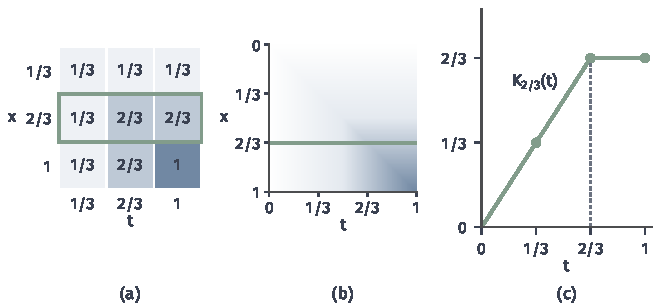
\includegraphics[width=112mm]{figures/04-spaces-measures-and-geometry/03-function-spaces/matplotlib/rkhs-kernel-as-matrix/figure.pdf}
  \caption{最小值核是一个连续下标的矩阵。(a)网格$\tfrac13,\tfrac23,1$上的矩阵$\bm K$，绿框是$x=\tfrac23$对应的行。(b)下标连成一片后的二元函数$\min(t,x)$，绿线是同一行。(c)沿绿线读出的函数就是核截面$K_{2/3}(t)=\min(t,\tfrac23)$，三个圆点是(a)中绿框内的三个数。}
  \label{fig:rkhs-kernel-as-matrix}
\end{BookInlineFigure}

类比有两处要留心。第一，有限维中$\bm K$与$\bm A$互逆，二者同样好用；无限维中通常只有$K$还是一个函数。式~\eqref{eq:rkhs-finite-difference-form}显示，网格加密时$\bm A$的元素以$1/h$的速度增长，它的极限不是二元函数，而是求导运算。所以无限维的内积一般不能用“矩阵元素”写出，我们只留下$K$。

第二，$\mathbb R^n$中每个向量都有有限长度，而函数空间中“有限长度”是实实在在的限制。$\mathbb K^X$中的绝大多数函数不属于$H$。核截面总在$H$中，标准单位向量的对应物，即只在$x$处有值的“尖峰”，却通常不在$H$中；这正是$L^2$上点值出问题的原因，读取坐标的向量在那里不存在。

\paragraph{两个例子中的核截面}

在$H_{\mathrm{aff}}$中，设$K_x=c+dt$，再生性质要求下式对一切$a,b$成立：
\[
\overline c\,a+\overline d\,b=a+bx .
\]
比较系数得$c=1$，$d=\overline x=x$。所以
\[
K_x(t)=1+xt,\qquad K(t,x)=1+tx ,
\]
称为仿射核。

图~\ref{fig:rkhs-reproducing-geometry}把这个计算画在系数平面上。核截面$K_x$对应向量$(1,x)$，读取$f=1+t$在$x=\tfrac12$处的值，就是计算$(1,1)$与$(1,\tfrac12)$的内积$1.5$。而$K_{-1}=(1,-1)$与$(1,1)$正交，对应$f(-1)=0$。函数在某点取零，几何上就是它与该点的核截面垂直。

\begin{BookInlineFigure}
  \centering
  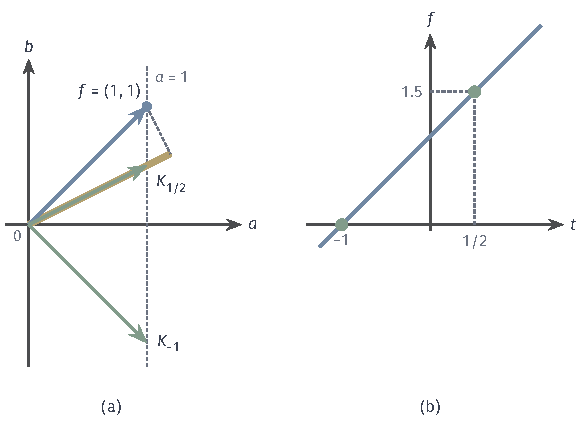
\includegraphics[width=99.4mm]{figures/04-spaces-measures-and-geometry/03-function-spaces/tikz/rkhs-reproducing-geometry/figure.pdf}
  \caption{仿射函数空间中再生性质的几何。(a)系数平面$(a,b)$与空间等距；蓝色向量是$f=1+t$，绿色向量是核截面$K_x=1+xt$，都落在虚线$a=1$上。黄色线段是$f$在$K_{1/2}$方向上的投影，其长度乘以$\lVert K_{1/2}\rVert$等于$f(1/2)=1.5$；$K_{-1}$与$f$垂直。(b)同一函数的图像，圆点标出$t=1/2$处的读数$1.5$与$t=-1$处的零点。}
  \label{fig:rkhs-reproducing-geometry}
\end{BookInlineFigure}

在$H_{\min}$中，式~\eqref{eq:rkhs-hmin-point-bound}的推导已经把$f(x)$写成了对$f'$的积分：
\[
f(x)=\int_0^1\mathbf 1_{[0,x]}(t)\,f'(t)\,\mathrm dt .
\]
只需找一个左端为零、导数为$\mathbf 1_{[0,x]}$的函数，它就是$K_x(t)=\min(t,x)$：在$[0,x]$上斜率为$1$，在$[x,1]$上保持常数$x$。

直接核对：
\[
\langle K_x,f\rangle_{H_{\min}}=\int_0^xf'(t)\,\mathrm dt=f(x) .
\]
称
\[
K(t,x)=\min(t,x)\qquad(t,x\in[0,1])
\]
为\term{最小值核}（minimum kernel）。它就是图~\ref{fig:rkhs-kernel-as-matrix}中的矩阵取遍全部下标的结果，式~\eqref{eq:rkhs-finite-difference-form}也随之成为$\int_0^1f'(t)^2\,\mathrm dt$。本章反复使用这个例子，因为它的空间、核截面和谱都可以精确算出。

\paragraph{再生核的基本性质}

核值是两个核截面的内积，内积的性质于是直接转化为核的性质。下面的定理列出其中最常用的几条。

\begin{theorem}[再生核的基本性质]
\label{thm:rkhs-kernel-properties}
设$H$是$X$上的RKHS，$K$为其再生核。则：
\begin{enumerate}
\item 共轭对称：对一切$x,y\in X$，$K(y,x)=\overline{K(x,y)}$；实值情形即$K(x,y)=K(y,x)$。
\item 正定性：对任意$n\geq1$、任意点$x_1,\ldots,x_n\in X$与$c_1,\ldots,c_n\in\mathbb K$，
\begin{equation}
\sum_{i,j=1}^n\overline{c_i}\,c_j\,K(x_i,x_j)=\Bigl\lVert\sum_{j=1}^nc_jK_{x_j}\Bigr\rVert_H^2\geq0 .
\label{eq:rkhs-kernel-positivity}
\end{equation}
\item 点评估的范数与核值的界：
\begin{equation}
\lVert\delta_x\rVert=\lVert K_x\rVert_H=\sqrt{K(x,x)},\qquad
\lvert K(x,y)\rvert\leq\sqrt{K(x,x)K(y,y)} .
\label{eq:rkhs-kernel-norm}
\end{equation}
\item 稠密性：核截面的有限线性组合全体$\operatorname{span}\{K_x:x\in X\}$在$H$中稠密。
\end{enumerate}
\end{theorem}

\begin{proof}
第1条来自内积的共轭对称：由式~\eqref{eq:rkhs-kernel-definition}，
\[
K(y,x)=\langle K_y,K_x\rangle=\overline{\langle K_x,K_y\rangle}=\overline{K(x,y)} .
\]

第2条把范数平方按内积对第一个变量共轭线性、对第二个变量线性展开：
\[
\Bigl\lVert\sum_jc_jK_{x_j}\Bigr\rVert^2=\sum_{i,j}\overline{c_i}\,c_j\,\langle K_{x_i},K_{x_j}\rangle=\sum_{i,j}\overline{c_i}\,c_j\,K(x_i,x_j).
\]

第3条中，Riesz表示给出$\lVert\delta_x\rVert=\lVert K_x\rVert$，而$\lVert K_x\rVert^2=\langle K_x,K_x\rangle=K(x,x)$；再对$\langle K_x,K_y\rangle$用Cauchy--Schwarz不等式，得到后一个不等式。

第4条用正交补判断。设$f\in H$与每个$K_x$正交，由再生性质，$f(x)=\langle K_x,f\rangle=0$对一切$x$成立，$f$是零函数。一个子空间的正交补只含零元时，它的闭包就是整个$H$（第~\ref{chap:function-inner-product-spaces}章的正交分解）。
\end{proof}

第2条中以$K(x_i,x_j)$为元素的矩阵$\bm G$是核截面组的\term{Gram矩阵}，在核的语境中也称\term{核矩阵}（kernel matrix）。把这个“无限大的矩阵”$K$限制到任意有限个下标，得到的子矩阵都半正定，这与上面的有限维样板一致。第1、2两条只涉及核，不涉及空间，下一节就把它们作为单独对二元函数的要求。

由第3条，单位球中的函数在$x$处的取值恰好填满半径$\sqrt{K(x,x)}$的圆盘（实值时是区间）：上界来自Cauchy--Schwarz不等式，取$f=K_x/\lVert K_x\rVert$即可达到。

所以前面关于统一常数的问题有了明确的答案。存在常数$C$使下式对一切$x$成立，
\[
\lvert f(x)\rvert\leq C\lVert f\rVert_H ,
\]
当且仅当$\sup_xK(x,x)<\infty$，最佳常数是$\sup_x\sqrt{K(x,x)}$。仿射核的对角值$1+x^2$在$\mathbb R$上无界，最小值核的对角值$x$不超过$1$，与前面直接得到的估计一致。

\section{从正定核构造空间}
\label{sec:rkhs-from-kernel}

上一节从空间出发得到核，并发现核的Gram矩阵总是半正定的。实际问题中往往反过来：人们先写下一个衡量两点相似程度的二元函数，再问它对应什么样的函数空间。

有限维中这个问题的答案已经知道。给定对称正定矩阵$\bm K$，令$\bm A=\bm K^{-1}$，就得到以$\bm K$为读坐标矩阵的内积空间。无限维中$\bm A$通常不存在，所以构造必须只用$\bm K$本身。本节证明，只要二元函数满足有限点组上的半正定条件，就存在唯一的RKHS以它为再生核。

构造分三步：先在核截面的有限线性组合上定义内积，并检查它不依赖于组合的写法；再处理长度为零的方向；最后完备化，并确认补进来的极限元素仍然是函数。

\subsection{正定核}
\label{sec:rkhs-pd-kernels}

定理~\ref{thm:rkhs-kernel-properties}的第1、2条只涉及核在有限个点上的值。把它们单独拿出来，就得到对二元函数的要求：把$K$看成下标取遍$X\times X$的矩阵，要求它的每个有限子矩阵都半正定。

\begin{definition}[正定核与严格正定核]
\label{def:rkhs-pd-kernel}
设$X$是非空集合，$K:X\times X\to\mathbb K$。若对任意$n\geq1$、任意点$x_1,\ldots,x_n\in X$与任意$c_1,\ldots,c_n\in\mathbb K$，
\begin{equation}
\sum_{i,j=1}^n\overline{c_i}\,c_j\,K(x_i,x_j)\geq0 ,
\label{eq:rkhs-pd-condition}
\end{equation}
并且在$\mathbb K=\mathbb R$时还有$K(x,y)=K(y,x)$，则称$K$为$X$上的\term{正定核}（positive definite kernel）。若进一步对任意\emph{互异}的点$x_1,\ldots,x_n$及不全为零的系数，上式严格大于零，则称$K$为\term{严格正定核}（strictly positive definite kernel）。
\end{definition}

用矩阵的语言，正定核要求每个Gram矩阵$\bm G=[K(x_i,x_j)]_{i,j}$都是Hermite半正定矩阵，严格正定核要求互异点组上的Gram矩阵都是正定矩阵，因而可逆。在复数情形，二次型对一切复系数取实值已经迫使$\bm G$是Hermite矩阵，所以不必另加对称条件；实数情形只用实系数检验，对称性必须单独要求。

“正定核”是通行的名称，但它只要求Gram矩阵\emph{半}正定，允许矩阵奇异。之所以要区分严格正定，是因为后文有限观测问题能否对任意数据求解，正取决于Gram矩阵是否可逆。定义中强调互异的点：若$x_1=x_2$，Gram矩阵的前两行相同，任何核的这个矩阵都奇异。

\paragraph{半正定但不严格正定的例子}

仿射核$K(x,y)=1+xy$由上一节的空间得到，所以是正定核。取三个互异点$-1,0,1$，Gram矩阵及其一个零向量为
\[
\bm G=\begin{bmatrix}2&1&0\\1&1&1\\0&1&2\end{bmatrix},\qquad
\bm G\begin{bmatrix}1\\-2\\1\end{bmatrix}=\bm 0 .
\]
对应的函数组合恰好是零函数：
\[
K_{-1}-2K_0+K_1=(1-t)-2+(1+t)=0 .
\]
原因是$H_{\mathrm{aff}}$只有二维，任意三个核截面必然线性相关。所以仿射核正定而不严格正定。

\paragraph{严格正定的例子}

\term{高斯核}（Gaussian kernel）是最常用的严格正定核：
\[
K_\sigma(x,y)=\exp\Bigl(-\frac{\lvert x-y\rvert^2}{2\sigma^2}\Bigr)\qquad(x,y\in\mathbb R).
\]
它的严格正定性可以直接证明。第~\ref{chap:fourier-transform}章算过Gauss函数的Fourier变换，把那里的结果作伸缩，下式对一切实数$u$成立：
\[
\exp\Bigl(-\frac{u^2}{2\sigma^2}\Bigr)=\int_{\mathbb R}\mathrm e^{\mathrm i\omega u}\,p_\sigma(\omega)\,\mathrm d\omega,\qquad
p_\sigma(\omega)=\frac{\sigma}{\sqrt{2\pi}}\mathrm e^{-\sigma^2\omega^2/2}.
\]

取互异的$x_1,\ldots,x_n$与系数$c_j$，令
\[
g(\omega)=\sum_jc_j\mathrm e^{-\mathrm i\omega x_j}.
\]
把$u=x_i-x_j$代入二次型，交换有限和与积分，被积函数恰好成为一个模平方：
\[
\sum_{i,j}\overline{c_i}\,c_j\,K_\sigma(x_i,x_j)=\int_{\mathbb R}\lvert g(\omega)\rvert^2\,p_\sigma(\omega)\,\mathrm d\omega\geq0 .
\]

若积分为零，由$p_\sigma>0$与$g$连续，$g$恒为零。对$g$在$\omega=0$处求$k$阶导数，$k=0,\ldots,n-1$，得到
\[
\sum_{j=1}^nc_j\,x_j^k=0 .
\]
这是系数矩阵为Vandermonde矩阵的齐次方程组，点互异时只有零解，所以$c_1=\cdots=c_n=0$。这就证明了高斯核严格正定。

在两个点$0,1$、$\sigma=1$上可以直接核对：Gram矩阵及其特征值为
\[
\begin{bmatrix}1&\mathrm e^{-1/2}\\\mathrm e^{-1/2}&1\end{bmatrix},\qquad
1\pm\mathrm e^{-1/2}\approx1.607,\ 0.393,
\]
两个特征值都为正。

图~\ref{fig:rkhs-gram-matrices}在五个点上比较这两种核。两者都是半正定矩阵，高斯核的五个特征值都为正，仿射核只有两个正特征值，其余为零。这幅图只检验了一个点组，严格正定性需要像上面那样对一切互异点组论证。

\begin{BookInlineFigure}
  \centering
  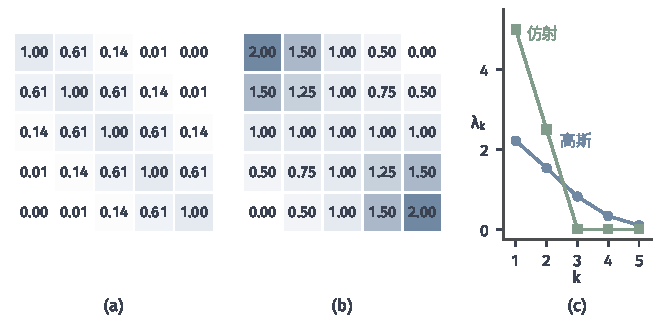
\includegraphics[width=112mm]{figures/04-spaces-measures-and-geometry/03-function-spaces/matplotlib/rkhs-gram-matrices/figure.pdf}
  \caption{点组$x=-1,-0.5,0,0.5,1$上的Gram矩阵。(a)高斯核（$\sigma=0.5$），颜色越深核值越大，数字保留两位小数（右上角的$0.00$实为$\mathrm e^{-8}\approx0.0003$）。(b)仿射核$1+xz$。(c)两个矩阵的特征值从大到小排列：高斯核为$2.217,1.531,0.820,0.333,0.099$，全为正；仿射核只有$5$与$2.5$两个正特征值。两种核都半正定，只有前者的矩阵可逆。}
  \label{fig:rkhs-gram-matrices}
\end{BookInlineFigure}

\subsection{核截面的有限线性组合}
\label{sec:rkhs-finite-combinations}

下面固定$X$上的一个正定核$K$。如果以$K$为再生核的空间存在，它必定含有全部核截面$K_x=K(\cdot,x)$，并且由式~\eqref{eq:rkhs-kernel-definition}，截面之间的内积只能是$\langle K_x,K_y\rangle=K(x,y)$。构造就从这两点出发。

\paragraph{有限维的样板：只用$\bm K$写内积}

先在有限维中看怎样不用逆矩阵写出内积。矩阵$\bm K$的列的线性组合形如$\bm K\bm c$。若$\bm K$可逆，把$\bm K\bm c$与$\bm K\bm d$代入内积，逆矩阵$\bm A$被消掉：
\[
\langle\bm K\bm c,\bm K\bm d\rangle_{\bm A}=\bm c^{\top}\bm K\bm A\bm K\bm d=\bm c^{\top}\bm K\bm d .
\]
最右端只含$\bm K$，$\bm K$奇异时照样有意义。这时同一个向量可以由不同的系数表示，$\bm K$的零向量就是长度为零的系数方向。下面的构造逐字重复这个想法。

\paragraph{半内积}

令$H_0=\operatorname{span}\{K_x:x\in X\}$，它的元素是有限和，也就是$X$上的函数：
\[
f=\sum_ia_iK_{x_i},\qquad f(t)=\sum_ia_iK(t,x_i).
\]
对这样的$f$与另一个元素$g=\sum_jb_jK_{y_j}$，按上述要求规定
\begin{equation}
\langle f,g\rangle_0=\sum_{i,j}\overline{a_i}\,b_j\,K(x_i,y_j).
\label{eq:rkhs-h0-inner}
\end{equation}
它对$g$线性、对$f$共轭线性，具有共轭对称性，并且由正定条件知$\langle f,f\rangle_0\geq0$。

问题在于，同一个函数可以有多种有限和表示，例如仿射核下$K_{-1}+K_1$与$2K_0$是同一个函数。必须先检查式~\eqref{eq:rkhs-h0-inner}的值不依赖于表示的选取。

固定$i$先对$j$求和，因为$g(x_i)=\sum_jb_jK(x_i,y_j)$，得到第一种写法。固定$j$先对$i$求和，并用$K(x_i,y_j)=\overline{K(y_j,x_i)}$，得到第二种写法：
\[
\langle f,g\rangle_0=\sum_i\overline{a_i}\,g(x_i)
=\sum_jb_j\,\overline{f(y_j)} .
\]
第一种写法只通过$g$的函数值依赖于$g$，第二种只通过$f$的函数值依赖于$f$。所以换掉$g$的表示不改变第一种写法，换掉$f$的表示不改变第二种写法，$\langle f,g\rangle_0$确实是两个\emph{函数}的量。

取$f=K_x$，第一种写法给出
\begin{equation}
\langle K_x,g\rangle_0=g(x)\qquad(g\in H_0),
\label{eq:rkhs-h0-reproducing}
\end{equation}
即再生性质在$H_0$上已经成立。

\paragraph{零范数方向的商}

现在看长度为零的方向。若把系数本身当作对象，即考虑有限支撑的系数族$a=(a_x)_{x\in X}$组成的线性空间$V$，并用式~\eqref{eq:rkhs-h0-inner}的右端定义$\langle a,b\rangle_V$，那么这只是一个半内积。仿射核的例子中，点$-1,0,1$上的系数$(1,-2,1)$非零，长度却为零。于是$\lVert a\rVert_V=\langle a,a\rangle_V^{1/2}$只是半范数，$d(a,b)=\lVert a-b\rVert_V$只是伪度量。

第~\ref{chap:metric-spaces}章对伪度量的处理是把零距离的点视为同一个点，作商空间。这里同样令
\[
N=\{a\in V:\lVert a\rVert_V=0\}.
\]
半内积的Cauchy--Schwarz不等式的证明只用到半正定性与线性，因此照样成立：
\[
\lvert\langle a,b\rangle_V\rvert\leq\lVert a\rVert_V\lVert b\rVert_V .
\]
由它可知，$a\in N$当且仅当$\langle a,b\rangle_V=0$对一切$b$成立，从而$N$是线性子空间，半内积下降到商空间$V/N$上成为真正的内积。

剩下的是把商空间与函数空间$H_0$对应起来。把系数$a$映为函数$f_a=\sum_xa_xK_x$，这个映射从$V$到$H_0$满射。记$e_t\in V$为只在$t$处取$1$、其余处取$0$的系数，则
\[
\langle e_t,a\rangle_V=\sum_xa_xK(t,x)=f_a(t),\qquad \lVert e_t\rVert_V^2=K(t,t).
\]
由半内积的Cauchy--Schwarz不等式，
\begin{equation}
\lvert f_a(t)\rvert=\lvert\langle e_t,a\rangle_V\rvert\leq\sqrt{K(t,t)}\,\lVert a\rVert_V .
\label{eq:rkhs-h0-point-bound}
\end{equation}

式~\eqref{eq:rkhs-h0-point-bound}说明，$a\in N$时$f_a$在每一点为零。反过来，$f_a\equiv0$时，
\[
\lVert a\rVert_V^2=\sum_x\overline{a_x}\,f_a(x)=0 .
\]
可见零范数的系数恰好是给出零函数的系数，商空间$V/N$与$H_0$一一对应，$\langle\cdot,\cdot\rangle_0$是$H_0$上真正的内积。把系数映成函数，恰好完成了零距离商。

\subsection{空间的完备化}
\label{sec:rkhs-completion}

$H_0$一般不完备。以最小值核为例，$H_0$由左端为零、在有限个节点处转折的连续折线组成，而下面这列折线的极限不是折线。取$m$个等距节点上核截面的平均：
\[
f_m=\frac1m\sum_{i=1}^mK_{i/m},\qquad K_{i/m}(t)=\min(t,\tfrac im).
\]
它的导数在第$k$段$(\tfrac{k-1}m,\tfrac km]$上等于$\tfrac{m-k+1}m$。

取$f(t)=t-t^2/2$，它的导数是$1-t$。在第$k$段上两个导数之差为$t-\tfrac{k-1}m$，所以
\[
\lVert f_m-f\rVert_{H_{\min}}^2=m\int_0^{1/m}u^2\,\mathrm du=\frac1{3m^2}.
\]
$(f_m)$在核范数下是Cauchy列，极限$t-t^2/2$属于$H_{\min}$，却不是折线，不在$H_0$中。下面补上这些极限，并确认它们仍然是$X$上的函数。

\paragraph{完备化与点值的极限}

由第~\ref{chap:metric-spaces}章，$H_0$有完备化$\overline{H_0}$，它由$H_0$中Cauchy列的等价类组成，$H_0$在其中稠密；内积沿Cauchy列取极限延拓过去，$\overline{H_0}$成为Hilbert空间。但完备化中的元素是抽象的等价类，还不是$X$上的函数，接下来要把它们变回函数。

点值估计~\eqref{eq:rkhs-h0-point-bound}正好提供这一步。若$(f_k)$是$H_0$中的Cauchy列，则
\[
\lvert f_k(x)-f_l(x)\rvert\leq\sqrt{K(x,x)}\,\lVert f_k-f_l\rVert_0 ,
\]
所以在每一点$f_k(x)$都是Cauchy数列，有确定的极限。两个等价的Cauchy列相差一列范数趋于零的函数，在每一点有相同的极限。用内积写出来，就是定义
\[
J:\overline{H_0}\to\mathbb K^X,\qquad (J\xi)(x)=\langle K_x,\xi\rangle_{\overline{H_0}} .
\]
若$f_k\to\xi$，则$f_k(x)=\langle K_x,f_k\rangle\to(J\xi)(x)$，所以$J\xi$就是逼近$\xi$的Cauchy列的逐点极限。由式~\eqref{eq:rkhs-h0-reproducing}，$J$在$H_0$上是恒等映射。

\paragraph{极限元素仍可识别为函数}

还剩一个危险：$\overline{H_0}$中两个不同的元素，会不会给出同一个函数？若是这样，函数之间就无法定义内积。等价地，要排除$\xi\neq0$而$J\xi$是零函数的情形。

若$\langle K_x,\xi\rangle=0$对一切$x$成立，则$\xi$与每个核截面正交，从而与它们的张成$H_0$正交。$H_0$在$\overline{H_0}$中稠密，所以$\xi$与整个空间正交，$\xi=0$。因此$J$是单射。

\begin{theorem}[由正定核确定再生核Hilbert空间]
\label{thm:rkhs-moore-aronszajn}
设$K$是非空集合$X$上的正定核。则存在唯一的RKHS，记为$H_K$，以$K$为其再生核。并且$H_0=\operatorname{span}\{K_x:x\in X\}$在$H_K$中稠密，$H_K$的每个元素都是$H_0$中某个Cauchy列的逐点极限。
\end{theorem}

\begin{proof}
先证存在性。令$H_K=J(\overline{H_0})$，规定
\[
\langle J\xi,J\eta\rangle_{H_K}=\langle\xi,\eta\rangle_{\overline{H_0}} .
\]
$J$是线性单射，这个定义良好，$J$成为等距同构，所以$H_K$是Hilbert空间；$J$的线性说明$H_K$中的加法和数乘就是逐点运算。

$J$在$H_0$上是恒等映射，故$K_x\in H_K$。对$f=J\xi$，由$J$的定义和等距性，
\[
f(x)=\langle K_x,\xi\rangle_{\overline{H_0}}=\langle JK_x,J\xi\rangle_{H_K}=\langle K_x,f\rangle_{H_K} .
\]
这就是以$K$为再生核的再生性质，点评估有界随之成立。稠密性与逐点极限的描述来自$H_0$在$\overline{H_0}$中稠密，以及上面关于$J$的讨论。

再证唯一性。设$H$是另一个以$K$为再生核的RKHS。$H$含有每个$K_x$，且$\langle K_x,K_y\rangle_H=K(x,y)$，所以$H_0\subseteq H$，两者在$H_0$上的内积一致。由定理~\ref{thm:rkhs-kernel-properties}的第4条，$H_0$在$H$中稠密。

任取$f\in H$及$H_0$中按$H$范数收敛到$f$的序列$f_k$。它是$H_0$中的Cauchy列，由再生性质逐点收敛到$f$。同一序列在$H_K$中收敛到其逐点极限，也就是$f$。所以$f\in H_K$，且
\[
\lVert f\rVert_{H_K}=\lim_k\lVert f_k\rVert_0=\lVert f\rVert_H .
\]
对调两个空间的角色，得$H=H_K$，再由极化恒等式知内积相同。
\end{proof}

这个结论通常称为Moore--Aronszajn定理\scite{aronszajn1950kernels}。图~\ref{fig:rkhs-construction-steps}用最小值核把构造的四个阶段画了出来。从此以后，“正定核”与“RKHS”可以互相确定：每个RKHS有唯一的再生核，每个正定核恰好是一个RKHS的再生核。

\begin{BookInlineFigure}
  \centering
  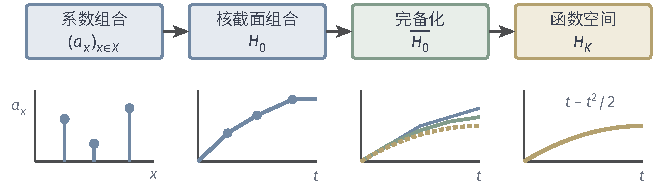
\includegraphics[width=111.1mm]{figures/04-spaces-measures-and-geometry/03-function-spaces/tikz/rkhs-construction-steps/figure.pdf}
  \caption{用最小值核走一遍由正定核构造$H_K$的四个阶段。第一栏是有限支撑的系数，二次型只给出半内积；第二栏把系数$(a_x)$变成函数$\sum_xa_xK_x$，这里是折线，零长度方向由此被商去；第三栏的蓝线、绿线是$m=2,4$时的平均折线$f_m$，虚线是它们在核范数下的极限；第四栏的$t-t^2/2$是该极限作为函数的样子，点值由Cauchy列逐点取极限得到。}
  \label{fig:rkhs-construction-steps}
\end{BookInlineFigure}

\paragraph{由最小值核重建$H_{\min}$}

以最小值核为例走一遍构造。核截面的导数是$\mathbf 1_{[0,x]}$，所以截面的内积可以写成导数的积分：
\[
\langle K_x,K_y\rangle_0=\min(x,y)=\int_0^1K_x'(t)\,K_y'(t)\,\mathrm dt .
\]
于是在$H_0$上$\lVert f\rVert_0=\lVert f'\rVert_{L^2}$。$H_0$中函数的导数恰好是区间上的阶梯函数，而阶梯函数在$L^2(0,1)$中稠密（第~\ref{chap:function-approximation}章）。于是完备化后的空间经由$f\mapsto f'$与$L^2(0,1)$等距同构，它就是上一节的$H_{\min}$。

这里唯一性起了作用：我们已经知道$H_{\min}$是以$\min(x,y)$为再生核的RKHS，定理~\ref{thm:rkhs-moore-aronszajn}保证从核出发构造的空间就是它，不必另作比较。

整个构造只用到集合$X$与核的正定性，没有用到测度或拓扑。所得的稠密性是在核范数意义下的，它不回答有限核截面组合能否逼近$H_K$之外的函数，这个问题留到第~\ref{sec:rkhs-section-span-approx}节。

\section{正定核的构造}
\label{sec:rkhs-kernel-constructions}

定理~\ref{thm:rkhs-moore-aronszajn}把问题归结为核的正定性，但直接检验一个二元函数的正定性并不方便：定义要求对一切有限点组和一切系数核验二次型。本节给出三条可操作的规则：把核写成特征向量的内积；对已知正定核作非负线性组合；对已知正定核作逐点乘积。每条规则都回到有限Gram矩阵的二次型来核验，最后用它们验证多项式核与高斯核。

\subsection{特征映射构造}
\label{sec:rkhs-feature-maps}

最常用的验证办法是把输入映到一个内积空间，再用像的内积定义核。二次型于是变成一个向量的长度平方，自然非负。

\begin{definition}[特征映射]
\label{def:rkhs-feature-map}
设$X$是非空集合，$\mathcal F$是Hilbert空间，$\Phi:X\to\mathcal F$是任意映射。称
\[
K(x,y)=\langle\Phi(x),\Phi(y)\rangle_{\mathcal F}\qquad(x,y\in X)
\]
为由$\Phi$给出的核，称$\Phi$为$K$的一个\term{特征映射}（feature map），$\mathcal F$为相应的特征空间（feature space）。
\end{definition}

由特征映射给出的核总是正定的：对任意点组与系数，
\[
\sum_{i,j}\overline{c_i}\,c_j\,K(x_i,x_j)=\Bigl\langle\sum_ic_i\Phi(x_i),\ \sum_jc_j\Phi(x_j)\Bigr\rangle_{\mathcal F}=\Bigl\lVert\sum_jc_j\Phi(x_j)\Bigr\rVert_{\mathcal F}^2\geq0 ,
\]
共轭对称性则来自内积本身。用矩阵写，若$\mathcal F=\mathbb K^d$，记$\bm\Phi$为第$i$行是$\Phi(x_i)^*$的$n\times d$矩阵，则Gram矩阵是$\bm\Phi\bm\Phi^*$。

反过来，每个正定核都有特征映射：取$\mathcal F=H_K$，$\Phi(x)=K_x$，则$\langle K_x,K_y\rangle_{H_K}=K(x,y)$。称它为\term{规范特征映射}（canonical feature map）。所以“$K$正定”与“$K$有某个特征映射”是等价的两种说法。

\paragraph{线性核与有限特征核}

在$\mathbb R^d$上，取$\Phi(\bm x)=\bm x$，得到\term{线性核}（linear kernel）$K(\bm x,\bm y)=\bm x^{\top}\bm y$。在$\mathbb R$上，展开平方可得
\[
(1+xy)^2=1+2xy+x^2y^2=\bigl\langle(1,\sqrt2\,x,x^2),\ (1,\sqrt2\,y,y^2)\bigr\rangle ,
\]
所以二次多项式核是三维特征向量的内积核。这类由有限个特征分量给出的核称为有限特征核，它们的Gram矩阵秩不超过特征维数，因而在点数超过特征维数时一定奇异。

\paragraph{特征维数与RKHS}

同一个核可以有许多不同的特征映射。仿射核$1+xy$既可以由$\Phi_1(x)=(1,x)\in\mathbb R^2$给出，也可以由$\Phi_2(x)=(1,x/\sqrt2,x/\sqrt2)\in\mathbb R^3$给出，因为$1+\tfrac{xy}{2}+\tfrac{xy}{2}=1+xy$。特征空间的维数和坐标都不同，核却相同，由核确定的RKHS也相同。所以特征维数不是空间的性质，RKHS中的函数及其范数要从核读出。

下面说明怎样从任何一个特征映射读出RKHS。给定$\Phi:X\to\mathcal F$，每个参数$w\in\mathcal F$确定一个函数
\[
f_w(x)=\langle\Phi(x),w\rangle_{\mathcal F}.
\]
令$V$为$\{\Phi(x):x\in X\}$张成的闭子空间，$P_V$为到$V$的正交投影。$w-P_Vw$与每个$\Phi(x)$正交，所以$f_w=f_{P_Vw}$：$V^\perp$中的参数分量对函数没有任何影响。

\begin{theorem}[特征映射给出的RKHS]
\label{thm:rkhs-feature-space}
设$\Phi:X\to\mathcal F$是正定核$K$的特征映射，$V$为$\Phi(X)$张成的闭子空间。则
\begin{equation*}
\begin{gathered}
H_K=\{f_w:w\in\mathcal F\},\\
\lVert f_w\rVert_{H_K}=\lVert P_Vw\rVert_{\mathcal F}=\min\{\lVert u\rVert_{\mathcal F}:u\in\mathcal F,\ f_u=f_w\} ,
\end{gathered}
\end{equation*}
并且$w\mapsto f_w$限制在$V$上是从$V$到$H_K$的等距同构。
\end{theorem}

\begin{proof}
线性映射$A:w\mapsto f_w$的核是$\{w:\langle\Phi(x),w\rangle=0,\ \forall x\}=V^\perp$，所以$A$在$V$上是单射，且$A(\mathcal F)=A(V)$。令$H=A(\mathcal F)$，规定$\langle Aw,Au\rangle_H=\langle P_Vw,P_Vu\rangle_{\mathcal F}$，则$A|_V$是等距同构，$H$作为闭子空间$V$的等距像是Hilbert空间，运算是逐点的。

令$k_x=A\Phi(x)$。因$\Phi(x)\in V$，有$\langle k_x,f_w\rangle_H=\langle\Phi(x),P_Vw\rangle=\langle\Phi(x),w\rangle=f_w(x)$；而$k_x(y)=\langle\Phi(y),\Phi(x)\rangle=K(y,x)$，即$k_x=K_x$。所以$H$是以$K$为再生核的RKHS，由定理~\ref{thm:rkhs-moore-aronszajn}的唯一性，$H=H_K$。最后，$f_u=f_w$当且仅当$u-w\in V^\perp$，此时$P_Vu=P_Vw$，而$\lVert u\rVert\geq\lVert P_Vu\rVert$，等号在$u\in V$时取得。
\end{proof}

定理的最后一个等式说明：在冗余的特征表示中，任意一个能给出$f$的参数，其长度只是$\lVert f\rVert_{H_K}$的上界；只有落在$V$中的参数，长度才等于函数的范数。

\begin{example}[冗余特征]
\label{ex:rkhs-redundant-features}
取$\Phi(x)=(x,x)\in\mathbb R^2$，核为$K(x,y)=2xy$。$V$是直线$\operatorname{span}\{(1,1)\}$，正交补方向是$(1,-1)$。参数$(2,0)$、$(1,1)$、$(0,2)$都给出同一函数$f(x)=2x$，长度分别为$2$、$\sqrt2$、$2$；由定理~\ref{thm:rkhs-feature-space}，$\lVert f\rVert_{H_K}=\sqrt2$，是$(2,0)$在$V$上的投影$(1,1)$的长度，见图~\ref{fig:rkhs-visible-parameters}。

直接核对：$H_K$由$f(x)=cx$组成，核截面$K_x(t)=2xt$，再生性质要求$\langle 2xt,ct\rangle=cx$，故$\langle at,ct\rangle_{H_K}=ac/2$，$\lVert 2x\rVert_{H_K}^2=4/2=2$，结果一致。特征空间是二维的，RKHS却是一维的。
\end{example}

\begin{figure}[!htb]
  \centering
  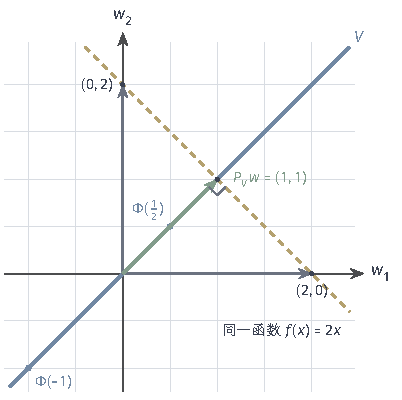
\includegraphics[width=68.1mm]{figures/02-abstract-mathematics/03-function-spaces/tikz/c5-visible-parameters/figure.pdf}
  \caption{冗余特征$\Phi(x)=(x,x)$的参数平面。各点的特征$\Phi(x)$都落在蓝色直线$V$上；黄色虚线上的参数都给出同一函数$f(x)=2x$。其中与$V$相交的$P_Vw=(1,1)$长度最短，为$\sqrt2$，这就是$\lVert f\rVert_{H_K}$；$(2,0)$与$(0,2)$长度为$2$，多出的部分来自对函数没有影响的$V^\perp$方向。}
  \label{fig:rkhs-visible-parameters}
\end{figure}

对仿射核的两个特征映射，$\Phi_1$的$V$是整个$\mathbb R^2$，所以$\lVert a+bt\rVert_{H_K}^2=a^2+b^2$，与第~\ref{sec:rkhs-evaluation-bounds}节一致。$\Phi_2$的$V$是$\operatorname{span}\{(1,0,0),(0,1,1)/\sqrt2\}$，参数$(a,b/\sqrt2,b/\sqrt2)$给出$a+bt$，长度同样是$\sqrt{a^2+b^2}$；参数$(a,\sqrt2\,b,0)$也给出同一函数，长度$\sqrt{a^2+2b^2}$却更大。

\subsection{非负线性组合}
\label{sec:rkhs-nonnegative-combinations}

特征映射适合验证可以写成内积的核。更多的核由几个已知核组合得到，只要组合方式保持正定性，就不必为每个新核重新寻找特征映射。最简单的组合是加权求和。

\begin{theorem}[非负线性组合]
\label{thm:rkhs-nonnegative-combination}
设$K_1,\ldots,K_m$是$X$上的正定核，$\alpha_1,\ldots,\alpha_m\geq0$是非负实数。则$K=\sum_l\alpha_lK_l$是$X$上的正定核。
\end{theorem}

\begin{proof}
固定点组与系数向量$\bm c$，记$\bm G_l$为$K_l$的Gram矩阵，则$K$的Gram矩阵是$\sum_l\alpha_l\bm G_l$，且
\[
\bm c^*\Bigl(\sum_l\alpha_l\bm G_l\Bigr)\bm c=\sum_l\alpha_l\,\bm c^*\bm G_l\bm c\geq0 ,
\]
因为每一项都是非负数与非负数之积。实数情形下对称性显然保持。
\end{proof}

用特征映射表达，若$\Phi_l$是$K_l$的特征映射，把$\sqrt{\alpha_l}\,\Phi_l(x)$依次拼接成直和空间$\mathcal F_1\oplus\cdots\oplus\mathcal F_m$中的一个向量，其内积正是$\sum_l\alpha_lK_l(x,y)$。例如仿射核$1+xy$是常数核$1$（特征为常数$1$）与线性核$xy$之和，拼接特征就是前面的$\Phi_1(x)=(1,x)$。

系数的符号不能任意改变。仿射核减去常数核$2$得到$xy-1$，它在$x=y=0$处的值为$-1$；而正定核在单点上的Gram矩阵是$1\times1$矩阵$[K(x,x)]$，必须非负。所以两个正定核之差一般不是正定核。复系数同样不行：$\mathrm iK$的对角值是纯虚数，二次型不再取实值。

\subsection{逐点乘积}
\label{sec:rkhs-pointwise-products}

第二种组合是逐点相乘。这时乘积核的Gram矩阵是两个Gram矩阵的逐元素乘积，正定性来自卷二的Schur乘积定理：两个同阶Hermite半正定矩阵的逐元素乘积仍是Hermite半正定矩阵，可参考\BookChapterRef{chap:normed-inner-product-spaces}{卷二第3章“赋范空间与内积空间”}。其机制是把两组向量的内积相乘，等于它们张量积之间的内积。

\begin{theorem}[逐点乘积]
\label{thm:rkhs-pointwise-product}
设$K_1,K_2$是同一集合$X$上的正定核。则$K(x,y)=K_1(x,y)K_2(x,y)$是$X$上的正定核。若$\Phi_1,\Phi_2$分别是$K_1,K_2$取值于$\mathbb K^{d_1},\mathbb K^{d_2}$的特征映射，则$\Phi_1(x)\otimes\Phi_2(x)\in\mathbb K^{d_1d_2}$是$K$的特征映射。
\end{theorem}

\begin{proof}
固定点组，$K$的Gram矩阵是$\bm G_1\odot\bm G_2$，由Schur乘积定理它是Hermite半正定矩阵，所以$K$正定。对特征映射，按坐标展开$\langle u\otimes v,u'\otimes v'\rangle=\sum_{k,l}\overline{u_kv_l}\,u_k'v_l'=\langle u,u'\rangle\langle v,v'\rangle$，取$u=\Phi_1(x)$、$v=\Phi_2(x)$、$u'=\Phi_1(y)$、$v'=\Phi_2(y)$即得。
\end{proof}

\paragraph{两条辅助规则}

验证常见的连续核，还需要两条与乘积相关的简单规则。第一条是函数缩放：对任意$g:X\to\mathbb K$，$g(x)\overline{g(y)}$是正定核，因为
\[
\sum_{i,j}\overline{c_i}\,c_j\,g(x_i)\overline{g(x_j)}=\Bigl\lvert\sum_i\overline{c_i}\,g(x_i)\Bigr\rvert^2\geq0 ;
\]
于是由定理~\ref{thm:rkhs-pointwise-product}，$g(x)\overline{g(y)}K(x,y)$对任意正定核$K$仍正定。第二条是逐点极限：若正定核$K^{(k)}$在每个$(x,y)$处收敛到$K(x,y)$，则$K$正定，因为每个有限二次型都是非负数的极限。

\paragraph{多项式核与高斯核}

由这几条规则可以验证常用的核。常数$c\geq0$是以$\sqrt c$为特征的核，所以$c+\bm x^{\top}\bm y$正定（定理~\ref{thm:rkhs-nonnegative-combination}），它的$p$次幂即\term{多项式核}（polynomial kernel）$(c+\bm x^{\top}\bm y)^p$也正定（定理~\ref{thm:rkhs-pointwise-product}反复使用）。

$\mathbb R^d$上的高斯核$K_\sigma(\bm x,\bm y)=\exp\bigl(-\lVert\bm x-\bm y\rVert_2^2/(2\sigma^2)\bigr)$分三步验证。先展开指数中的平方：
\[
\exp\Bigl(-\frac{\lVert\bm x-\bm y\rVert_2^2}{2\sigma^2}\Bigr)
=g(\bm x)\,g(\bm y)\,\exp\Bigl(\frac{\bm x^{\top}\bm y}{\sigma^2}\Bigr),\qquad
g(\bm x)=\exp\Bigl(-\frac{\lVert\bm x\rVert_2^2}{2\sigma^2}\Bigr).
\]
再看中间因子：部分和$\sum_{k=0}^N(\bm x^{\top}\bm y)^k/(k!\,\sigma^{2k})$是线性核各次幂的非负组合，因而正定；指数级数逐点收敛，由逐点极限规则，$\exp(\bm x^{\top}\bm y/\sigma^2)$正定。最后由函数缩放规则乘上$g(\bm x)g(\bm y)$。这样得到的是正定性；严格正定性是更强的性质，第~\ref{sec:rkhs-pd-kernels}节已经说明它需要另外的论证。

\paragraph{运算在核截面上的效果}

核的运算直接作用在核截面上：和核的截面是两个截面之和，乘积核的截面是两个截面之积。图~\ref{fig:rkhs-kernel-operations}在$x=0.4$处比较仿射核与高斯核（$\sigma=0.3$）。和核的截面在仿射趋势上叠加了一个局部隆起；乘积核的截面仍集中在$x$附近，但被仿射因子$1+0.4t$拉得右高左低。所以乘积核对应空间中的函数同时带有两种核的特点：局部性来自高斯因子，倾斜来自仿射因子。

\begin{figure}[!htb]
  \centering
  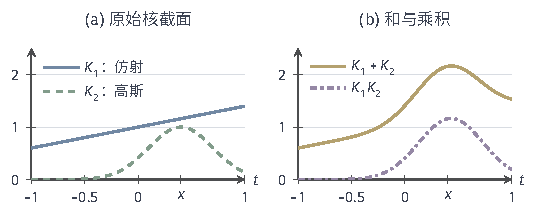
\includegraphics[width=90.7mm]{figures/02-abstract-mathematics/03-function-spaces/tikz/c5-kernel-operations/figure.pdf}
  \caption{核运算在核截面上的效果，固定$x=0.4$，$t\in[-1,1]$。(a)~仿射核截面$1+0.4t$与高斯核截面（$\sigma=0.3$）；(b)~两者之和与逐点乘积。和核的截面是两个截面相加，乘积核的截面是两个截面相乘，仍保持以$x$为中心的局部形状。}
  \label{fig:rkhs-kernel-operations}
\end{figure}

本节的规则都从已知的核或已知的特征出发。还有一种重要的特征来自核本身的谱：在定义域上加入测度后，核积分算子的特征函数给出一组按特征值加权的特征，这要用到算子的谱理论，在第~\ref{sec:rkhs-mercer}节另行构造。

\section{最小范数插值}
\label{sec:rkhs-min-norm-interpolation}

现在回到第~\ref{sec:rkhs-recovery}节的精确插值问题，把候选空间取为RKHS。固定$X$上的RKHS $H$及其再生核$K$，取观测位置$x_1,\ldots,x_n\in X$（暂不要求互异）和读数$\bm y\in\mathbb K^n$，要找$f\in H$使$f(x_i)=y_i$对每个$i$成立。

这个问题要分两步回答。第一步判断数据能否由$H$中的函数实现；若不能，谈论“最好的插值”没有意义。第二步在可行函数中选出范数最小的一个。两步都依赖同一个正交分解：把$H$分成读数能看见的有限维部分与读数完全看不见的部分。

\subsection{观测映射}
\label{sec:rkhs-observation-map}

把$n$个读数合在一起，得到线性映射
\[
S:H\to\mathbb K^n,\qquad Sf=\bigl(f(x_1),\ldots,f(x_n)\bigr)^{\top},
\]
称为\term{观测映射}（observation map）。精确插值就是解方程$Sf=\bm y$。由再生性质，$Sf$的第$i$个分量是$\langle K_{x_i},f\rangle$，所以$S$是有界线性映射，并且$\lVert Sf\rVert_2^2\leq\bigl(\sum_iK(x_i,x_i)\bigr)\lVert f\rVert_H^2$。

\paragraph{伴随与Gram矩阵}

$\mathbb K^n$取标准内积$\langle\bm c,\bm d\rangle=\bm c^*\bm d$。对任意$\bm c\in\mathbb K^n$，
\[
\langle\bm c,Sf\rangle=\sum_i\overline{c_i}\,f(x_i)=\sum_i\overline{c_i}\,\langle K_{x_i},f\rangle_H=\Bigl\langle\sum_ic_iK_{x_i},\ f\Bigr\rangle_H ,
\]
所以$S$的伴随把系数映成核截面的组合：$S^*\bm c=\sum_ic_iK_{x_i}$。这类函数的读数和内积都可以用Gram矩阵$\bm G_{i,j}=K(x_i,x_j)$计算：
\begin{equation}
S(S^*\bm c)=\bm G\bm c,\qquad
\langle S^*\bm c,S^*\bm d\rangle_H=\bm c^*\bm G\bm d,\qquad
SS^*=\bm G .
\label{eq:rkhs-gram-calculus}
\end{equation}
第一式的第$i$个分量是$\sum_jc_jK(x_i,x_j)$，第二式由$\langle K_{x_i},K_{x_j}\rangle=K(x_i,x_j)$展开得到。于是在核截面的张成空间内，函数的全部计算都化为$n$维向量与$n\times n$矩阵的计算。注意$\bm c^*\bm G\bm c$才是函数的范数平方，系数的欧氏长度$\lVert\bm c\rVert_2$一般与函数范数无关。

\paragraph{秩与线性相关}

$\bm G$的秩恰好是核截面$K_{x_1},\ldots,K_{x_n}$张成空间的维数。因为$\bm G$是Hermite半正定矩阵，$\bm c^*\bm G\bm c=0$当且仅当$\bm G\bm c=\bm 0$；而由式~\eqref{eq:rkhs-gram-calculus}，$\bm c^*\bm G\bm c=\lVert S^*\bm c\rVert_H^2$。所以$\ker\bm G=\ker S^*$，即$\bm G\bm c=\bm 0$恰好描述核截面之间的线性关系，由秩—零度公式即得上述结论。

$\bm G$奇异有三种典型来源。一是重复观测：若$x_1=x_2$，则$K_{x_1}=K_{x_2}$，$\bm G$的前两行相同。二是核截面所在的空间维数不够：仿射核在$-1,0,1$上的Gram矩阵以$(1,-2,1)^{\top}$为零向量，因为二维空间中三个截面必然线性相关。三是退化的观测点：最小值核满足$K_0=\min(\cdot,0)=0$，$H_{\min}$中所有函数在$0$处取零，含有$x=0$的观测点组，Gram矩阵有一整行为零。

\begin{example}[最小值核的观测映射]
\label{ex:rkhs-hmin-observation}
在$H_{\min}$中取$x_1,x_2,x_3=\tfrac13,\tfrac23,1$，Gram矩阵为
\[
\bm G=\frac13\begin{bmatrix}1&1&1\\1&2&2\\1&2&3\end{bmatrix},\qquad
\det\bm G=\frac1{27}\neq0 .
\]
三个核截面线性无关，它们的组合$S^*\bm c=\sum_jc_j\min(\cdot,x_j)$恰好是左端为零、只在$\tfrac13,\tfrac23$处转折的连续折线：在三段上的斜率依次为$c_1+c_2+c_3$、$c_2+c_3$、$c_3$。
\end{example}

\subsection{观测零空间}
\label{sec:rkhs-observation-null-space}

读数看不见的函数组成$S$的核
\[
N=\ker S=\{f\in H:f(x_1)=\cdots=f(x_n)=0\},
\]
称为\term{观测零空间}（observation null space）。$S$有界，所以$N$是闭子空间。记$M=\operatorname{span}\{K_{x_1},\ldots,K_{x_n}\}$，它是$S^*$的像，有限维因而闭。下面的定理说明这两个子空间互为正交补。

\begin{theorem}[观测零空间的正交补]
\label{thm:rkhs-observation-null-space}
在上述记号下，$N=M^\perp$，$N^\perp=M$，从而$H=M\oplus N$。记$P$为到$M$的正交投影，则对一切$f\in H$，$S(Pf)=Sf$且$\lVert Pf\rVert_H\leq\lVert f\rVert_H$。两个函数$f,g$在全部观测点上读数相同，当且仅当$f-g\in N$，也当且仅当$Pf=Pg$。
\end{theorem}

\begin{proof}
$f\in N$当且仅当$\langle K_{x_i},f\rangle=0$对每个$i$成立，即$f$与$M$的每个生成元正交，这就是$N=M^\perp$。$M$是闭子空间，所以$N^\perp=M^{\perp\perp}=M$，正交分解$H=M\oplus N$由第~\ref{chap:inner-product-spaces}章的投影定理给出。$f-Pf\in N$说明$S(f-Pf)=0$；勾股定理给出$\lVert f\rVert^2=\lVert Pf\rVert^2+\lVert f-Pf\rVert^2$。最后，$Sf=Sg$等价于$f-g\in N$，而由正交分解，这又等价于$P(f-g)=0$。
\end{proof}

所以有限个点值恰好确定投影$Pf$，余项$f-Pf$完全看不见：它在每个观测点取零，不论多大都不改变任何读数。

\begin{example}[折线与观测零空间的正交性]
\label{ex:rkhs-hmin-null-space}
继续例~\ref{ex:rkhs-hmin-observation}。$N$由$H_{\min}$中在$\tfrac13,\tfrac23,1$处取零的函数组成，例如$\sin(3k\pi x)$（$k=1,2,\ldots$），所以$N$是无限维的。$M$是左端为零、以$\tfrac13,\tfrac23$为节点的折线。

正交性可以直接验证：设$h\in M$在第$k$段上的斜率为$s_k$，$g\in N$，则
\[
\langle h,g\rangle_{H_{\min}}=\int_0^1h'g'=\sum_{k=1}^3s_k\bigl(g(\tfrac k3)-g(\tfrac{k-1}3)\bigr)=0 ,
\]
因为$g$在四个节点$0,\tfrac13,\tfrac23,1$上都取零。在这个例子中，$Pf$就是过原点和三个观测点的折线插值。
\end{example}

定理~\ref{thm:rkhs-observation-null-space}还有一个更一般的推论。若某个准则只通过读数$Sf$依赖于$f$，再加上一项随$\lVert f\rVert_H$增大的惩罚，那么把$f$换成$Pf$不改变前者、不增大后者，最优函数总可以取在有限维空间$M$中，即写成$\sum_jc_jK_{x_j}$的形式。这就是带损失与正则项的函数拟合中表示定理的结构依据，可参考\BookChapterRef{chap:function-fitting-regularization}{卷五第10章“函数拟合与正则化”}。本章只讨论精确插值这一特殊情形。

\subsection{约束相容性}
\label{sec:rkhs-consistency}

给定读数$\bm y$，第一步要判断是否存在$f\in H$满足$Sf=\bm y$。不是任意数据都能被插值：在重复观测点上给出两个不同的读数，任何函数都无法同时满足。下面的定理把可行性写成矩阵条件。

\begin{theorem}[插值约束的相容性]
\label{thm:rkhs-consistency}
存在$f\in H$使$Sf=\bm y$，当且仅当$\bm y$属于$\bm G$的像，也当且仅当$\bm d^*\bm y=0$对一切$\bm d\in\ker\bm G$成立。
\end{theorem}

\begin{proof}
若$Sf=\bm y$，由定理~\ref{thm:rkhs-observation-null-space}，$\bm y=S(Pf)$，而$Pf\in M$可写成$S^*\bm c$，于是$\bm y=SS^*\bm c=\bm G\bm c$。反过来，若$\bm y=\bm G\bm c$，则$f=S^*\bm c$满足$Sf=\bm y$。$\bm G$是Hermite矩阵，其像是$\ker\bm G$的正交补，这给出第二个等价条件。
\end{proof}

当$\bm G$可逆时，像是整个$\mathbb K^n$，任意数据都可以插值；特别地，严格正定核在互异观测点上总是如此。当$\bm G$奇异时，数据必须满足$\ker\bm G$给出的线性关系。仿射核在$-1,0,1$上，$\ker\bm G$由$(1,-2,1)^{\top}$张成，相容条件是$y_1-2y_2+y_3=0$，即三个数据点共线。读数$(0,1,0)$不满足它，所以没有仿射函数通过这三点；这与第~\ref{sec:rkhs-finite-feature-space}节例~\ref{ex:rkhs-polynomial-features}的第1种情形是同一现象，只是那里用设计矩阵的列空间来判断。重复观测$x_1=x_2$时$(1,-1,0,\ldots,0)^{\top}\in\ker\bm G$，相容条件是$y_1=y_2$；$H_{\min}$中在$0$处观测时，相容条件是该读数为零。

还要区分“没有插值函数”与“插值函数不止一个”，二者由不同的对象决定。前者取决于$\bm y$是否落在$\bm G$的像中；后者取决于观测零空间$N$是否非零，与$\bm G$是否可逆无关。仿射核在$-1,0,1$上$\bm G$奇异，但三个截面已经张成整个$H_{\mathrm{aff}}$，$N=\{0\}$，相容数据确定唯一的函数。$H_{\min}$中三个观测点给出可逆的$\bm G$，任何数据都可行，$N$却是无限维的，可行函数有无穷多个。所以不能把$\bm G$奇异理解为插值不唯一，也不能把$\bm G$可逆理解为函数被唯一确定。

\subsection{最小范数解}
\label{sec:rkhs-min-norm-solution}

数据相容时，可行函数组成仿射集$f_0+N$，其中$f_0$是任意一个可行函数。第~\ref{sec:rkhs-finite-feature-space}节在有限特征空间中遇到解不唯一时，卷二的做法是选欧氏长度最小的系数；在RKHS中，自然的做法是选范数最小的函数。

\begin{theorem}[最小范数插值]
\label{thm:rkhs-min-norm-interpolation}
设$\bm y$属于$\bm G$的像，$\bm c$是方程$\bm G\bm c=\bm y$的任意一个解，令
\[
f^+=S^*\bm c=\sum_{j=1}^nc_jK_{x_j},\qquad f^+(x)=\sum_{j=1}^nc_jK(x,x_j).
\]
则$f^+$不依赖于解$\bm c$的选取，它是$M$中唯一满足$Sf=\bm y$的函数；对任意满足$Sg=\bm y$的$g\in H$，
\begin{equation}
\lVert g\rVert_H^2=\lVert f^+\rVert_H^2+\lVert g-f^+\rVert_H^2 ,
\label{eq:rkhs-min-norm-pythagoras}
\end{equation}
所以$f^+$是唯一的最小范数可行函数，并且$\lVert f^+\rVert_H^2=\bm c^*\bm y=\bm y^*\bm G^{\dagger}\bm y$，其中$\bm G^{\dagger}$是Moore--Penrose伪逆。
\end{theorem}

\begin{proof}
由式~\eqref{eq:rkhs-gram-calculus}，$Sf^+=\bm G\bm c=\bm y$，所以$f^+$可行。若$\bm c'$是另一个解，则$\bm G(\bm c-\bm c')=\bm 0$，由上一小节$S^*(\bm c-\bm c')=0$，两组系数给出同一函数。$M$中两个读数相同的函数之差属于$M\cap N=\{0\}$，这给出$M$中的唯一性。

对可行的$g$，$g-f^+\in N$，而$f^+\in M=N^\perp$，勾股定理即为式~\eqref{eq:rkhs-min-norm-pythagoras}，等号仅在$g=f^+$时成立。最后，$\lVert f^+\rVert^2=\bm c^*\bm G\bm c=\bm c^*\bm y$；取$\bm c=\bm G^{\dagger}\bm y$是方程的一个解（$\bm y$在$\bm G$的像中），代入并用$\bm G^{\dagger}$为Hermite矩阵，得$\bm y^*\bm G^{\dagger}\bm y$。
\end{proof}

称$f^+$为数据的\term{最小范数插值}（minimum-norm interpolation）。由定理~\ref{thm:rkhs-observation-null-space}，它也是任意可行函数在$M$上的投影。整个求解只需要核在观测点上的值：解一个$n\times n$的线性方程，再用核截面组合出函数。

\paragraph{系数不唯一与函数唯一}

定理区分了两种唯一性。$\bm G$奇异时，方程$\bm G\bm c=\bm y$的解组成$\bm c_0+\ker\bm G$，系数不唯一；但$\ker\bm G$中的系数给出零函数，所以函数$f^+$唯一。伪逆从全部解中挑出欧氏长度最小的系数，这只是选了一种写法，与函数范数最小是两回事。

仿射核在$-1,0,1$上，取相容数据$\bm y=(0,1,2)^{\top}$。$\bm c=(0,0,1)^{\top}$是一个解，全部解为$(s,-2s,1+s)^{\top}$。无论$s$取何值，$f^+=sK_{-1}-2sK_0+(1+s)K_1=1+t$，范数平方$\bm c^*\bm y=-2s+2(1+s)=2=1^2+1^2$。

\begin{example}[最小值核的折线插值]
\label{ex:rkhs-hmin-interpolation}
在例~\ref{ex:rkhs-hmin-observation}的观测点上，取$q(x)=4x(1-x)$的读数$\bm y=(\tfrac89,\tfrac89,0)^{\top}$。由定理~\ref{thm:rkhs-min-norm-interpolation}与例~\ref{ex:rkhs-hmin-null-space}，$f^+$是过原点和三个数据点的折线，三段斜率依次为$\tfrac83,0,-\tfrac83$。对照例~\ref{ex:rkhs-hmin-observation}中的斜率公式，得$\bm c=(\tfrac83,\tfrac83,-\tfrac83)^{\top}$。

代回检验$\bm G\bm c=\bm y$：第一行$\tfrac13\cdot\tfrac83=\tfrac89$，第二行$\tfrac13(\tfrac83+\tfrac{16}3-\tfrac{16}3)=\tfrac89$，第三行$\tfrac13(\tfrac83+\tfrac{16}3-8)=0$。范数为$\lVert f^+\rVert^2=\bm c^{\top}\bm y=\tfrac{128}{27}$，也等于折线导数的平方积分$2\cdot\tfrac13\cdot\tfrac{64}{9}$。而$\lVert q\rVert_{H_{\min}}^2=\int_0^1(4-8x)^2\,\mathrm dx=\tfrac{16}3=\tfrac{144}{27}$，由式~\eqref{eq:rkhs-min-norm-pythagoras}，$\lVert q-f^+\rVert^2=\tfrac{16}{27}$。
\end{example}

最小范数插值只回答了“在可行函数中选哪一个”。它在测点之间与真实函数相差多少，取决于真实函数在$N$中的分量，这是读数看不见的部分。下一节在已知目标函数的前提下研究这种表示误差，并看它怎样随子空间的扩大而变化。

\section{有限维子空间逼近}
\label{sec:rkhs-finite-subspaces}

上一节从读数出发，目标函数未知，问题是在可行函数中选一个。本节换一个角度：目标函数$f\in H$已知，或者至少它与若干固定函数的内积可以算出，我们只允许用一个有限维子空间$V\subseteq H$中的函数来表示它。问题变成表示误差：$V$中离$f$最近的函数是谁，误差有多大，$V$逐步扩大后误差能否趋于零。

在Hilbert空间中，离$f$最近的元素就是正交投影$P_Vf$，误差为$\lVert f-P_Vf\rVert_H$（第~\ref{chap:function-inner-product-spaces}章）。RKHS的额外结构是，这个范数误差还能控制每一点的误差，而控制的系数只依赖于核与子空间，不依赖于$f$。

\begin{theorem}[子空间的再生核与逐点误差]
\label{thm:rkhs-subspace-error}
设$V$是RKHS $H$的闭子空间，$P_V$为到$V$的正交投影。则$V$带着$H$的内积是RKHS，其再生核为$K_V(x,y)=\langle P_VK_x,P_VK_y\rangle_H$；并且对一切$f\in H$与$x\in X$，
\begin{equation}
\lvert f(x)-(P_Vf)(x)\rvert\leq\sqrt{K(x,x)-K_V(x,x)}\ \lVert f-P_Vf\rVert_H .
\label{eq:rkhs-subspace-pointwise}
\end{equation}
\end{theorem}

\begin{proof}
对$g\in V$，$g(x)=\langle K_x,g\rangle=\langle P_VK_x,g\rangle$，所以$V$中$x$处的核截面是$P_VK_x$，再生核为式中所写。

令$r=f-P_Vf\in V^\perp$。$P_VK_x\in V$与$r$正交，所以
\[
r(x)=\langle K_x,r\rangle=\langle K_x-P_VK_x,r\rangle .
\]
用Cauchy--Schwarz不等式，并由勾股定理计算第一个因子：
\[
\lVert K_x-P_VK_x\rVert^2=\lVert K_x\rVert^2-\lVert P_VK_x\rVert^2=K(x,x)-K_V(x,x).
\]
这就是式~\eqref{eq:rkhs-subspace-pointwise}。
\end{proof}

式~\eqref{eq:rkhs-subspace-pointwise}右端的第一个因子是核截面$K_x$中不能由$V$表示的部分的长度，它只取决于核与子空间；第二个因子是$f$本身的表示误差。下面分别考察两类有限子空间：由核截面张成的子空间，以及由一般有限特征张成的子空间。

\subsection{核截面张成空间的逼近}
\label{sec:rkhs-section-span-approx}

取有限点组$Z=\{x_1,\ldots,x_n\}$，$V=M_Z=\operatorname{span}\{K_x:x\in Z\}$。由上一节，$P_{M_Z}f$就是$f$在$Z$上读数的最小范数插值，只需$f$的点值就能算出。这时式~\eqref{eq:rkhs-subspace-pointwise}中的第一个因子记为$P_Z(x)$，称为\term{核插值幂函数}（power function）。

$P_{M_Z}K_x$是$K_x$读数$\bm k_Z(x)=(K(x_1,x),\ldots,K(x_n,x))^{\top}$的最小范数插值，由定理~\ref{thm:rkhs-min-norm-interpolation}，
\begin{equation}
P_Z(x)^2=K(x,x)-\bm k_Z(x)^*\bm G^{\dagger}\bm k_Z(x).
\label{eq:rkhs-power-function}
\end{equation}
用矩阵的话说，这是$\bm K$关于观测下标的Schur补的对角元。它在每个观测点处为零，在观测点之间随间隔增大而增大。

\paragraph{点集决定的稠密性}

定理~\ref{thm:rkhs-kernel-properties}已经说明，全部核截面的组合在$H$中稠密，所以任何$f\in H$都能被有限个截面的组合任意逼近。实际中可选的位置往往受限，例如只能在一个点集$D\subseteq X$上放置截面。这时稠密性由下面的条件刻画。

\begin{theorem}[限定点集的核截面稠密性]
\label{thm:rkhs-dense-sections}
设$D\subseteq X$。则$\operatorname{span}\{K_x:x\in D\}$在$H$中稠密，当且仅当$H$中在$D$上处处为零的函数只有零函数。
\end{theorem}

\begin{proof}
由再生性质，$f$与每个$K_x$（$x\in D$）正交，当且仅当$f$在$D$上处处为零。一个子空间在Hilbert空间中稠密，当且仅当与它正交的元素只有零元。
\end{proof}

这个条件同时涉及核与点集。若$X$是度量空间且$K$连续，由再生性质与Cauchy--Schwarz不等式，
\[
\lvert f(x)-f(y)\rvert\leq\lVert f\rVert_H\lVert K_x-K_y\rVert_H ,
\]
其中核截面之差的长度可由核直接算出：
\[
\lVert K_x-K_y\rVert_H^2=K(x,x)+K(y,y)-2\operatorname{Re}K(x,y) .
\]
它随$y\to x$趋于零，所以$H$中的函数都连续。连续函数在稠密集上为零就处处为零，于是对连续核，任意稠密点集$D$上的截面都在$H$中稠密。

若核不连续，稠密的点集未必足够。取$X=[0,1]$上的离散核：$x=y$时$K(x,y)=1$，否则为$0$。这是“无限大的单位矩阵”，对应的RKHS是$\ell^2([0,1])$，即只在至多可数个点上非零且平方可和的函数。取$D$为$[0,1]$中的有理数，单点示性函数$\mathbf 1_{\{x_0\}}$（$x_0$为无理数）在$D$上为零而非零，所以$D$上的截面不稠密。核的连续性让读数在相邻位置之间传递信息，点集的稠密性才能发挥作用。

\begin{example}[最小值核的均匀节点]
\label{ex:rkhs-hmin-grid}
取步长$h=\tfrac1m$，在$H_{\min}$中取节点$Z_m=\{\tfrac1m,\tfrac2m,\ldots,1\}$。$P_{Z_m}f$是$f$的折线插值，其导数在每个小区间上等于$f'$在该区间上的平均。

对$q(x)=4x(1-x)$，$q'=4-8x$在每个长为$h$的区间上与其平均之差是斜率为$-8$、中点为零的线性函数，因此
\[
\lVert q-P_{Z_m}q\rVert_{H_{\min}}^2=m\int_{-h/2}^{h/2}(8u)^2\,\mathrm du=\frac{16h^2}{3}.
\]
$m=3$时为$\tfrac{16}{27}$，与例~\ref{ex:rkhs-hmin-interpolation}一致，并随$h\to0$趋于零。

幂函数也可以直接算出。设$x$落在小区间$[x_{k-1},x_k]$中，记$a=x-x_{k-1}$，$b=x_k-x$。$K_x-P_{Z_m}K_x$是$\min(\cdot,x)$减去它的折线插值，只在这个小区间上非零，斜率先为$b/h$、再为$-a/h$。把导数平方积分，
\[
P_{Z_m}(x)^2=a\cdot\frac{b^2}{h^2}+b\cdot\frac{a^2}{h^2}=\frac{ab}{h}.
\]
最大值$h/4$在区间中点取得。
\end{example}

\paragraph{RKHS范数误差与其他范数下的误差}

以上的误差都在$H$的范数下度量。若$\kappa^2=\sup_xK(x,x)<\infty$，由点评估界，
\[
\sup_x\lvert f(x)-g(x)\rvert\leq\kappa\lVert f-g\rVert_H ,
\]
所以$H$范数下的逼近蕴含一致逼近。反过来不成立。$H_{\min}$中$f_k(x)=\sin(k\pi x)/k$满足$\sup\lvert f_k\rvert\leq1/k$，而它的核范数不趋于零：
\[
\lVert f_k\rVert_{H_{\min}}^2=\int_0^1\pi^2\cos^2(k\pi x)\,\mathrm dx=\frac{\pi^2}2 .
\]
$H$范数还计入了函数的振荡，比一致范数更强。

另一个问题是用核截面去逼近$H$之外的函数，例如$[0,1]$上一个给定的连续函数$g$。这时误差只能在一致范数等较弱的范数下度量，能否任意逼近取决于$H$在相应函数空间中是否稠密，这是核本身的性质。仿射核的空间是二维的，在$C[-1,1]$中是闭子空间，不能一致逼近$\lvert x\rvert$。$H_{\min}$中的函数都在$0$处为零，只能一致逼近满足$g(0)=0$的连续函数。

高斯核的RKHS限制到紧集上以后，在该紧集的连续函数空间中按一致范数稠密，这类核称为\term{通用核}（universal kernel）。证明需要用到一致逼近的稠密性判据或测度的Fourier表示，篇幅较长，读者可查阅相关的核方法专著。它的含义是：只要节点选得足够多，高斯核截面的组合能在一致范数下逼近紧集上任意给定的连续函数。

所以核与点集各有分工。核决定$H$中有哪些函数、$H$能在多大范围内逼近外部函数，以及点值能否在相邻位置之间传递；点集决定所选截面能否充分利用$H$，即在$H$内部是否稠密。

\subsection{有限特征表示}
\label{sec:rkhs-finite-features}

核截面子空间的好处是坐标可以由点值读出，但它未必是表示给定函数类的最经济方式。另一种做法是在$H$中直接选定$m$个线性无关的函数$e_1,\ldots,e_m$作为特征，令$V=\operatorname{span}\{e_1,\ldots,e_m\}$，坐标预算就是$m$。

\paragraph{投影的计算}

记$\bm B$为特征在$H$内积下的Gram矩阵，元素为$\langle e_k,e_l\rangle_H$，它可逆。对$f\in H$，记$\bm b$为以$\langle e_k,f\rangle_H$为分量的向量。投影$P_Vf=\sum_la_le_l$的系数由正交条件确定：
\[
\langle e_k,f-P_Vf\rangle=0\qquad(k=1,\ldots,m),
\]
也就是$\bm B\bm a=\bm b$。误差由勾股定理得到：
\begin{equation}
\lVert f-P_Vf\rVert_H^2=\lVert f\rVert_H^2-\bm b^*\bm B^{-1}\bm b .
\label{eq:rkhs-feature-projection-error}
\end{equation}

对$V$的再生核，把$f=K_y$代入，$\bm b_k=\langle e_k,K_y\rangle=\overline{e_k(y)}$。记$\bm e(x)=(e_1(x),\ldots,e_m(x))^{\top}$，得到
\begin{equation}
K_V(x,y)=\bm e(x)^{\top}\bm B^{-1}\overline{\bm e(y)} .
\label{eq:rkhs-feature-subspace-kernel}
\end{equation}

与核截面相比，一般特征的坐标需要内积$\langle e_k,f\rangle_H$，它们一般不是点值读数。取$e_k=K_{x_k}$时，$\bm b_k=f(x_k)$，$\bm B$就是Gram矩阵$\bm G$，这时投影只需读数，这正是核截面的特殊之处。显式特征则可以利用对目标函数类的先验了解，用更少的坐标达到更小的误差。

\begin{example}[两个多项式特征]
\label{ex:rkhs-hmin-polynomial-features}
在$H_{\min}$中取$e_1=x$，$e_2=x^2$，它们都在$0$处为零。由$\langle f,g\rangle=\int_0^1f'g'$，
\[
\bm B=\begin{bmatrix}1&1\\1&\tfrac43\end{bmatrix},\qquad
\lVert a x+bx^2\rVert_{H_{\min}}^2=a^2+2ab+\tfrac43b^2 .
\]
$q(x)=4x-4x^2$本身属于$V$，两个坐标就给出零误差；例~\ref{ex:rkhs-hmin-interpolation}用三个核截面，误差却是$\sqrt{16/27}\approx0.77$。另一方面，这组特征只对二次多项式有利，换成振荡的目标函数，它未必比均匀节点的核截面更好。
\end{example}

\paragraph{有限特征核不是原核}

有限特征还可以用来定义一个新核。把例~\ref{ex:rkhs-hmin-polynomial-features}的特征排成向量$(x,x^2)$，按欧氏内积得到有限特征核$\widetilde K(x,y)=xy+x^2y^2$。由定理~\ref{thm:rkhs-feature-space}，$H_{\widetilde K}$与$V$含有同样的函数，范数却是$a^2+b^2$，与$H_{\min}$中的$a^2+2ab+\tfrac43b^2$不同。

$V$作为$H_{\min}$子空间的正确的核由式~\eqref{eq:rkhs-feature-subspace-kernel}给出。先求逆，再代入：
\[
\bm B^{-1}=\begin{bmatrix}4&-3\\-3&3\end{bmatrix},\qquad
K_V(x,y)=4xy-3xy^2-3x^2y+3x^2y^2 .
\]
它在对角线上满足$K_V(x,x)\leq K(x,x)=x$，例如$K_V(\tfrac12,\tfrac12)=\tfrac7{16}<\tfrac12$。由式~\eqref{eq:rkhs-subspace-pointwise}，任意$f\in H_{\min}$在$\tfrac12$处的投影误差不超过$\tfrac14\lVert f-P_Vf\rVert$。差$K-K_V$是$V^\perp$的再生核，只有$V=H$时才为零。

所以有限特征近似不应自动理解为原核的精确表示。特征的欧氏内积给出的是另一个空间的几何，只有按$H$的Gram矩阵加权，才得到原空间中子空间的核；即使如此，它也只代表原空间的一部分。

\section{Mercer谱表示}
\label{sec:rkhs-mercer}

到目前为止，RKHS的全部结构都只由核决定，没有用到测度。本节在定义域上加入一个参考测度，用核作积分核得到积分算子，再借助紧自伴算子的谱理论，把核写成特征函数的展开。这个展开给出RKHS的一组标准正交坐标，也给出一种由核本身确定的有限特征：保留前若干个谱方向。

全节使用下面的标准条件：$X$是紧度量空间，$K$是$X\times X$上连续的正定核，$\mu$是$X$上的有限正Borel测度，并且具有\term{全支撑}（full support），即$X$的每个非空开集测度为正。记$\kappa^2=\max_{x\in X}K(x,x)$，它有限，因为连续函数在紧集上有最大值。

\subsection{核积分算子}
\label{sec:rkhs-integral-operator}

在上述条件下定义\term{核积分算子}（kernel integral operator）
\[
(T_Kf)(x)=\int_XK(x,y)\,f(y)\,\mathrm d\mu(y),\qquad f\in L^2(\mu).
\]
$L^2(\mu)$取内积$\langle f,g\rangle_{L^2}=\int_X\overline f\,g\,\mathrm d\mu$。下面依次核验$T_K$的紧性、自伴性与正性，它们是使用谱定理所需的全部条件。

\paragraph{紧性、自伴性与像的连续性}

$K$连续且$X$紧，所以$\lvert K\rvert\leq\kappa^2$有界，又$\mu$有限，于是$K\in L^2(\mu\otimes\mu)$。第~\ref{chap:linear-operators}章说明，平方可积核给出的积分算子是Hilbert--Schmidt算子，因而是紧算子；由$K(y,x)=\overline{K(x,y)}$，交换积分次序得$\langle g,T_Kf\rangle_{L^2}=\langle T_Kg,f\rangle_{L^2}$，所以$T_K$自伴。

$T_K$的像比一般的$L^2$等价类好得多：对任意$g\in L^2(\mu)$，$T_Kg$是处处有定义的连续函数。事实上，由Cauchy--Schwarz不等式，
\[
\lvert(T_Kg)(x)-(T_Kg)(x')\rvert\leq\mu(X)^{1/2}\sup_{y\in X}\lvert K(x,y)-K(x',y)\rvert\,\lVert g\rVert_{L^2},
\]
而$K$在紧集$X\times X$上一致连续，右端随$x'\to x$趋于零。

\paragraph{积分算子的正性}

自伴只说明$\langle f,T_Kf\rangle$是实数，不说明它非负。正性来自核的正定性，但二者的联系需要一个逼近论证：正定性只涉及有限点组，积分则是连续的累计。

\begin{lemma}[正定连续核给出正算子]
\label{lem:rkhs-positive-operator}
在本节条件下，对一切$f\in L^2(\mu)$，
\[
\langle f,T_Kf\rangle_{L^2}=\iint_{X\times X}\overline{f(x)}\,K(x,y)\,f(y)\,\mathrm d\mu(x)\,\mathrm d\mu(y)\geq0 .
\]
\end{lemma}

\begin{proof}
先设$f$连续。给定$\varepsilon>0$，函数$(x,y)\mapsto\overline{f(x)}K(x,y)f(y)$在紧集上一致连续，取$\delta>0$使两点距离小于$\delta$时它的变化小于$\varepsilon$。用有限个半径$\delta/2$的开球覆盖$X$，再依次去掉重叠部分，得到$X$的有限Borel划分$A_1,\ldots,A_N$，每块直径小于$\delta$；在每块中任取一点$x_i$，令$c_i=f(x_i)\mu(A_i)$。在$A_i\times A_j$上用常数$\overline{f(x_i)}K(x_i,x_j)f(x_j)$代替被积函数，得
\[
\Bigl\lvert\langle f,T_Kf\rangle-\sum_{i,j}\overline{c_i}\,c_j\,K(x_i,x_j)\Bigr\rvert\leq\varepsilon\,\mu(X)^2 .
\]
中间的和是点组$x_1,\ldots,x_N$上Gram矩阵的二次型，非负；令$\varepsilon\to0$即得$\langle f,T_Kf\rangle\geq0$。

对一般的$f\in L^2(\mu)$，连续函数在$L^2(\mu)$中稠密（紧度量空间上的有限Borel测度，见第~\ref{chap:function-approximation}章），而$f\mapsto\langle f,T_Kf\rangle$在$L^2$中连续，非负性保持到极限。
\end{proof}

\paragraph{再生关系与积分算子的区别}

核在这里扮演两种角色，不应混淆。在再生关系$f(x)=\langle K_x,f\rangle_H$中，核截面读取的是$f$在单个点的值，内积是$H$的内积，不涉及任何测度。在积分算子中，$K$对整条函数作加权累计，结果依赖于参考测度：同一个核配上不同的$\mu$，得到不同的算子。

以仿射核$K(x,y)=1+xy$为例，取$X=[-1,1]$。在$\mathrm d\mu=\mathrm dx/2$下，
\[
T_K1=\int_{-1}^1(1+xy)\,\frac{\mathrm dy}{2}=1,\qquad
T_Kx=\int_{-1}^1(1+xy)\,y\,\frac{\mathrm dy}{2}=\frac x3 ,
\]
与$1$、$x$都正交的函数被映为零。若改用$\mathrm d\mu=\mathrm dx$，算子整体变为原来的两倍。核没有变，算子随测度改变。

\subsection{核的谱展开}
\label{sec:rkhs-spectral-expansion}

至此，$T_K$是复Hilbert空间$L^2(\mu)$上的紧、自伴、正算子。第~\ref{chap:operator-spectra}章的谱定理给出：非零特征值都是正数，至多可数，按重数重复排列为$\lambda_1\geq\lambda_2\geq\cdots>0$，只能在零处聚集；相应的标准正交特征函数$\phi_j$构成$(\ker T_K)^\perp$的标准正交基，并且$T_Kf=\sum_j\lambda_j\langle\phi_j,f\rangle_{L^2}\phi_j$在$L^2$范数下成立。特征函数的个数可以有限，也可以无限。

\paragraph{特征函数的连续代表}

特征函数起初只是$L^2$等价类。若$T_K\phi=\lambda\phi$且$\lambda>0$，则$\phi=\lambda^{-1}T_K\phi$几乎处处成立，右端是连续函数，所以$\phi$有连续代表，以下总取这个代表。全支撑保证这个代表唯一：两个连续函数若几乎处处相等，使它们不相等的点组成开集，测度为零，由全支撑只能是空集。

若$\mu$没有全支撑，例如$X=[0,1]$而$\mu$只是$[0,\tfrac12]$上的Lebesgue测度，那么在$(\tfrac12,1]$上任意改动的函数仍是同一个$L^2$元素，积分算子的特征函数无法确定函数在测度支撑之外的取值，下面的逐点展开也就无从谈起。

\paragraph{Mercer定理}

一般紧自伴算子的谱定理只给出算子作用在$L^2$范数下的展开，第~\ref{chap:operator-spectra}章也指出，由此得到的核展开只在乘积空间的$L^2$意义下收敛。在本节的条件下，可以得到核本身的逐点、一致展开，这就是\term{Mercer定理}（Mercer theorem）\scite{mercer1909functions}。

\begin{theorem}[Mercer定理]
\label{thm:rkhs-mercer}
设$X$是紧度量空间，$K$是$X\times X$上连续的正定核，$\mu$是$X$上全支撑的有限正Borel测度。设$\lambda_j>0$与连续的$\phi_j$是$T_K$的全部正特征值与$L^2(\mu)$标准正交特征函数。则
\begin{equation}
K(x,y)=\sum_j\lambda_j\,\phi_j(x)\,\overline{\phi_j(y)}\qquad(x,y\in X),
\label{eq:rkhs-mercer}
\end{equation}
级数在$X\times X$上绝对且一致收敛；并且$\sum_j\lambda_j=\int_XK(x,x)\,\mathrm d\mu(x)<\infty$。
\end{theorem}

\begin{proof}
第一步，对角线上的部分和有界。令$K^{(m)}(x,y)=K(x,y)-\sum_{j\leq m}\lambda_j\phi_j(x)\overline{\phi_j(y)}$，它连续，对应的积分算子满足$\langle f,T^{(m)}f\rangle=\sum_{j>m}\lambda_j\lvert\langle\phi_j,f\rangle\rvert^2\geq0$。若某点$K^{(m)}(x_0,x_0)<0$（对角值是实数），由连续性存在$x_0$的开邻域$U$使$\operatorname{Re}K^{(m)}<0$在$U\times U$上成立。取$f=\mathbf 1_U$，全支撑给出$\mu(U)>0$，于是实数$\langle f,T^{(m)}f\rangle=\iint_{U\times U}\operatorname{Re}K^{(m)}<0$，矛盾。所以对一切$m$与$x$，
\[
\sum_{j\leq m}\lambda_j\lvert\phi_j(x)\rvert^2\leq K(x,x)\leq\kappa^2 .
\]

第二步，固定$x$识别极限。由Cauchy--Schwarz不等式与第一步，
\[
\sum_{j=p}^q\lambda_j\lvert\phi_j(y)\phi_j(x)\rvert\leq\Bigl(\sum_{j=p}^q\lambda_j\lvert\phi_j(x)\rvert^2\Bigr)^{1/2}\kappa ,
\]
右端括号中的级数收敛，所以$S(y,x)=\sum_j\lambda_j\phi_j(y)\overline{\phi_j(x)}$关于$y$一致收敛，$S(\cdot,x)$连续。另一方面，$\langle\phi_j,K(\cdot,x)\rangle_{L^2}=\overline{(T_K\phi_j)(x)}=\lambda_j\overline{\phi_j(x)}$，与$S(\cdot,x)$的系数相同。所以连续函数$h=K(\cdot,x)-S(\cdot,x)$与每个$\phi_j$正交，属于$\ker T_K$；$T_Kh$连续且几乎处处为零，由全支撑处处为零，从而$\int\overline{h}\,K(\cdot,x)\,\mathrm d\mu=\overline{(T_Kh)(x)}=0$。又$\int\overline h\,S(\cdot,x)\,\mathrm d\mu=\sum_j\lambda_j\overline{\phi_j(x)}\langle h,\phi_j\rangle=0$，两式相减得$\int\lvert h\rvert^2\,\mathrm d\mu=0$。由全支撑与连续性，$h\equiv0$，即式~\eqref{eq:rkhs-mercer}逐点成立。

第三步，一致收敛。在对角线上，连续函数$R_m(x)=K(x,x)-\sum_{j\leq m}\lambda_j\lvert\phi_j(x)\rvert^2$随$m$单调下降并逐点趋于零。对任意$\varepsilon>0$，闭集$\{R_m\geq\varepsilon\}$随$m$递减且交为空集，由$X$的紧性，其中某一个已是空集，所以$R_m\to0$一致成立（这就是Dini定理的论证）。再由第二步的Cauchy--Schwarz估计，$\sum_{j>m}\lambda_j\lvert\phi_j(x)\phi_j(y)\rvert\leq\sqrt{R_m(x)R_m(y)}\leq\max R_m$，得到$X\times X$上的绝对一致收敛。最后对对角线逐项积分（一致收敛且$\mu$有限），$\int K(x,x)\,\mathrm d\mu=\sum_j\lambda_j\int\lvert\phi_j\rvert^2\,\mathrm d\mu=\sum_j\lambda_j$。
\end{proof}

比较两种结论：一般紧自伴算子只有$L^2$意义下的谱展开，特征函数只是等价类；Mercer定理在核连续、正定且测度全支撑的条件下，给出核本身的逐点、一致展开，其中每个$\phi_j$都取连续代表。零特征值方向不出现在展开~\eqref{eq:rkhs-mercer}中，下文任何形如“除以$\lambda_j$”的公式都只在正谱方向上使用。

\paragraph{两个核的谱}

仿射核在$[-1,1]$、$\mathrm dx/2$下，由上一小节的计算，正特征值为$\lambda_1=1$、$\lambda_2=\tfrac13$，标准正交特征函数为$\phi_1=1$、$\phi_2=\sqrt3\,x$。Mercer展开只有两项：$1+\tfrac13\cdot3xy=1+xy$；迹为$1+\tfrac13=\int_{-1}^1(1+x^2)\,\tfrac{\mathrm dx}{2}=\tfrac43$。零空间是与$1,x$正交的全部函数，例如$x^2-\tfrac13$，它是无限维的，却不出现在核的展开中。

最小值核在$[0,1]$、Lebesgue测度下有无穷多个正特征值，而且可以精确算出。对连续的$\phi$，
\[
(T_K\phi)(x)=\int_0^xy\,\phi(y)\,\mathrm dy+x\int_x^1\phi(y)\,\mathrm dy ,
\]
右端两次可微，$(T_K\phi)'(x)=\int_x^1\phi$，$(T_K\phi)''=-\phi$，并且$(T_K\phi)(0)=0$，$(T_K\phi)'(1)=0$。所以$T_K\phi=\lambda\phi$（$\lambda>0$）等价于边值问题$\lambda\phi''=-\phi$，$\phi(0)=0$，$\phi'(1)=0$，其解为$\phi(x)=\sin(\omega x)$，其中$\omega=\lambda^{-1/2}$且$\cos\omega=0$。归一化后
\[
\lambda_j=\frac1{\omega_j^2},\qquad \phi_j(x)=\sqrt2\,\sin(\omega_jx),\qquad \omega_j=\Bigl(j-\frac12\Bigr)\pi,\quad j=1,2,\ldots
\]
同样的推导说明$T_K\phi=0$迫使$\phi=-(T_K\phi)''=0$，零空间平凡，这些$\phi_j$构成$L^2(0,1)$的标准正交基。迹的检验：$\sum_j\lambda_j=\sum_j\tfrac{4}{(2j-1)^2\pi^2}=\tfrac12=\int_0^1x\,\mathrm dx$。

图~\ref{fig:rkhs-mercer-spectrum}画出最小值核的前三个特征函数，并比较三种核的特征值衰减：最小值核按$j^{-2}$衰减，$\sigma=0.5$的高斯核衰减得快得多，仿射核只有两个正特征值。核越光滑，积分算子越强烈地压低高频方向；这里只作为数值观察，不作为一般定理使用。图中的特征函数记作$\psi_j$，即本节的$\phi_j$。

\begin{figure}[!htb]
  \centering
  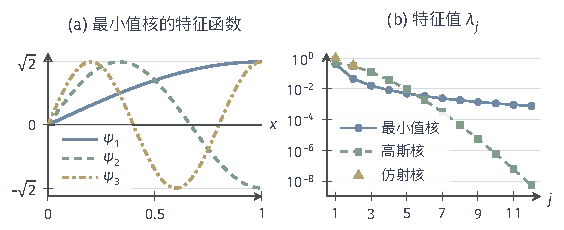
\includegraphics[width=95.5mm]{figures/02-abstract-mathematics/03-function-spaces/tikz/c5-mercer-spectrum/figure.pdf}
  \caption{Mercer特征函数与特征值衰减。(a)~最小值核在$[0,1]$、Lebesgue测度下的前三个特征函数$\psi_j=\sqrt2\sin((j-\frac12)\pi x)$，它们在$0$处为零、在$1$处导数为零；(b)~特征值（对数纵轴）：最小值核$\lambda_j=((j-\frac12)\pi)^{-2}$；高斯核（$\sigma=0.5$，$[-1,1]$，$\mathrm dz/2$）的特征值由40点Gauss--Legendre求积离散计算；仿射核只有$1$与$1/3$两个正特征值。}
  \label{fig:rkhs-mercer-spectrum}
\end{figure}

\subsection{RKHS中的谱坐标}
\label{sec:rkhs-spectral-coordinates}

Mercer展开把核写成了一族加权特征的内积：令$\Phi(x)=\bigl(\sqrt{\lambda_j}\,\overline{\phi_j(x)}\bigr)_j\in\ell^2$，则$\langle\Phi(x),\Phi(y)\rangle_{\ell^2}=\sum_j\lambda_j\phi_j(x)\overline{\phi_j(y)}=K(x,y)$。代入定理~\ref{thm:rkhs-feature-space}，就能读出RKHS在谱坐标下的形式。

\begin{theorem}[RKHS的谱表示]
\label{thm:rkhs-spectral-norm}
在定理~\ref{thm:rkhs-mercer}的条件下：
\begin{enumerate}
\item $\{\sqrt{\lambda_j}\,\phi_j\}$是$H_K$的标准正交基；
\item 函数$f:X\to\mathbb K$属于$H_K$，当且仅当存在数列$(a_j)$满足$\sum_j\lvert a_j\rvert^2/\lambda_j<\infty$，且$f(x)=\sum_ja_j\phi_j(x)$对一切$x$成立。此时级数在$X$上绝对一致收敛，$a_j=\langle\phi_j,f\rangle_{L^2(\mu)}$，并且
\begin{equation}
\lVert f\rVert_{L^2(\mu)}^2=\sum_j\lvert a_j\rvert^2,\qquad \lVert f\rVert_{H_K}^2=\sum_j\frac{\lvert a_j\rvert^2}{\lambda_j}.
\label{eq:rkhs-two-norms}
\end{equation}
\end{enumerate}
\end{theorem}

\begin{proof}
由定理~\ref{thm:rkhs-mercer}，$\lVert\Phi(x)\rVert^2=K(x,x)<\infty$，$\Phi$是$K$的特征映射，对应的函数为$f_w(x)=\langle\Phi(x),w\rangle=\sum_jw_j\sqrt{\lambda_j}\,\phi_j(x)$。先证$\Phi(X)$张成的闭子空间是整个$\ell^2$。设$w\in\ell^2$与每个$\Phi(x)$正交，即$\sum_jw_j\sqrt{\lambda_j}\phi_j(x)=0$对一切$x$成立。系数$w_j\sqrt{\lambda_j}$平方可和，同一级数在$L^2(\mu)$中收敛，其$L^2$极限有一个子列几乎处处收敛到它，所以$L^2$极限为零；由$\phi_j$的标准正交性，$w_j\sqrt{\lambda_j}=0$，即$w=0$。

于是由定理~\ref{thm:rkhs-feature-space}，$w\mapsto f_w$是从$\ell^2$到$H_K$的等距同构，单位向量$e_j$映为$\sqrt{\lambda_j}\phi_j$，这证明第1条。令$a_j=\sqrt{\lambda_j}\,w_j$，条件$w\in\ell^2$就是$\sum_j\lvert a_j\rvert^2/\lambda_j<\infty$，且$\lVert f_w\rVert_{H_K}^2=\sum_j\lvert w_j\rvert^2$。一致收敛来自
\[
\Bigl\lvert\sum_{j>m}a_j\phi_j(x)\Bigr\rvert\leq\Bigl(\sum_{j>m}\frac{\lvert a_j\rvert^2}{\lambda_j}\Bigr)^{1/2}\Bigl(\sum_{j>m}\lambda_j\lvert\phi_j(x)\rvert^2\Bigr)^{1/2}\leq\kappa\Bigl(\sum_{j>m}\frac{\lvert a_j\rvert^2}{\lambda_j}\Bigr)^{1/2} .
\]
一致收敛的级数也在$L^2(\mu)$中收敛到同一函数，由标准正交性得$a_j=\langle\phi_j,f\rangle_{L^2}$与$\lVert f\rVert_{L^2}^2=\sum_j\lvert a_j\rvert^2$。
\end{proof}

\paragraph{两种范数的坐标权重}

式~\eqref{eq:rkhs-two-norms}说明，同一组谱坐标$a_j$在两种范数中得到不同的权重：$L^2$范数对每个坐标一视同仁，RKHS范数把第$j$个坐标的平方放大$1/\lambda_j$倍。$L^2$中的单位方向$\phi_j$在$H_K$中的长度是$\lambda_j^{-1/2}$，$H_K$中真正的单位方向是$\sqrt{\lambda_j}\phi_j$。由于$\lambda_j\to0$，特征值小的方向在RKHS范数中代价很高。

对最小值核，$1/\lambda_j=\omega_j^2$，$\lVert f\rVert_{H_{\min}}^2=\sum_j\omega_j^2\lvert a_j\rvert^2$，这正是$\lVert f'\rVert_{L^2}^2$在余弦基$\sqrt2\cos(\omega_jx)$下的展开。图~\ref{fig:rkhs-norm-weights}中，$f=\phi_1$与$g=\phi_1+0.1\phi_8$的图像几乎重合，$\lVert f-g\rVert_{L^2}=0.1$；但$\lVert f-g\rVert_{H_{\min}}=0.1\,\omega_8=0.75\pi\approx2.36$，比$\lVert f\rVert_{H_{\min}}=\omega_1\approx1.57$还大。高频的小波纹带来很大的导数。

\begin{figure}[!htb]
  \centering
  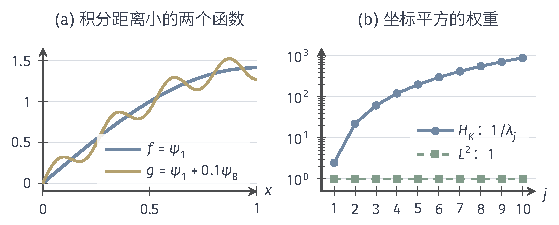
\includegraphics[width=94.6mm]{figures/02-abstract-mathematics/03-function-spaces/tikz/c5-norm-weights/figure.pdf}
  \caption{最小值核下两种范数的谱权重（图中$\psi_j$即正文的$\phi_j$）。(a)~$f=\psi_1$与$g=\psi_1+0.1\psi_8$，$\psi_j=\sqrt2\sin((j-\frac12)\pi x)$；两者的$L^2$距离为$0.1$，核范数距离却约为$2.36$。(b)~谱坐标平方在两种范数中的权重：$L^2$中恒为$1$，$H_K$中为$1/\lambda_j=((j-\frac12)\pi)^2$（对数纵轴），随$j$平方增长。}
  \label{fig:rkhs-norm-weights}
\end{figure}

\paragraph{只使用非零特征方向}

定理~\ref{thm:rkhs-spectral-norm}对$H_K$的成员提出两项要求：作为$L^2$元素，函数没有零特征值方向的分量；谱坐标的加权平方和有限。两项要求可以分别不满足。仿射核下，$x^2=\tfrac13\phi_1+(x^2-\tfrac13)$含有零空间分量$x^2-\tfrac13$，所以不在$H_{\mathrm{aff}}$中。最小值核下零空间平凡，但常数$1$的谱坐标为$a_j=\sqrt2/\omega_j$，$\sum_j\lvert a_j\rvert^2=1$有限，$\sum_j\lvert a_j\rvert^2/\lambda_j=\sum_j2$却发散；常数$1$在$L^2$中有谱展开，却不属于$H_{\min}$，这与$H_{\min}$要求$f(0)=0$相符。

\paragraph{谱坐标依赖测度，RKHS范数不依赖}

仍取仿射核，把$[-1,1]$上的测度从$\mathrm dx/2$换成$\mathrm dx$，特征值变为$2$与$\tfrac23$，标准正交特征函数变为$1/\sqrt2$与$\sqrt{3/2}\,x$。对$f=a+bx$，新的谱坐标为$a_1=\sqrt2\,a$，$a_2=\sqrt{2/3}\,b$，于是
\[
\frac{\lvert a_1\rvert^2}{\lambda_1}+\frac{\lvert a_2\rvert^2}{\lambda_2}=\frac{2a^2}{2}+\frac{2b^2/3}{2/3}=a^2+b^2 ,
\]
与原来的RKHS范数相同；而$L^2$范数平方从$a^2+b^2/3$变成了$2a^2+2b^2/3$。一般地，由定理~\ref{thm:rkhs-moore-aronszajn}，$H_K$的内积只由核决定；测度提供的是一组正交坐标和积分意义下的误差度量。

\subsection{Mercer谱特征的截断}
\label{sec:rkhs-spectral-truncation}

谱坐标给出一种由核与测度共同确定的有限特征：按非增的特征值保留前$N$个非零谱方向$\phi_1,\ldots,\phi_N$，令$V_N=\operatorname{span}\{\phi_1,\ldots,\phi_N\}$，把$f=\sum_ja_j\phi_j$截断为$f_N=\sum_{j\leq N}a_j\phi_j$。因为$\phi_j$在$L^2(\mu)$与$H_K$两种内积下都两两正交，$f_N$同时是$f$在$V_N$上的$L^2$投影与$H_K$投影。

\paragraph{两种尾和}

由式~\eqref{eq:rkhs-two-norms}，两种范数下的截断误差都是系数的尾和，只是权重不同：
\begin{equation}
\lVert f-f_N\rVert_{H_K}^2=\sum_{j>N}\frac{\lvert a_j\rvert^2}{\lambda_j},\qquad
\lVert f-f_N\rVert_{L^2(\mu)}^2=\sum_{j>N}\lvert a_j\rvert^2 .
\label{eq:rkhs-tail-sums}
\end{equation}
若$T_K$只有$r$个非零特征值（有限秩），则$H_K=V_r$是$r$维的，保留全部$r$个非零方向即可精确表示$H_K$中的每个函数，例如仿射核取$N=2$。下面考虑无穷多个非零特征值的情形。

\paragraph{单位球上的$L^2$误差}

对$j>N$有$\lambda_j\leq\lambda_{N+1}$，所以
\begin{equation}
\lVert f-f_N\rVert_{L^2(\mu)}^2=\sum_{j>N}\lambda_j\cdot\frac{\lvert a_j\rvert^2}{\lambda_j}\leq\lambda_{N+1}\lVert f-f_N\rVert_{H_K}^2\leq\lambda_{N+1}\lVert f\rVert_{H_K}^2 .
\label{eq:rkhs-tail-comparison}
\end{equation}
因此对RKHS单位球中的全部函数，$L^2$平方误差有统一的上界$\lambda_{N+1}$，随$N\to\infty$趋于零。这个界不能改进：$f=\sqrt{\lambda_{N+1}}\phi_{N+1}$的RKHS范数为$1$，$L^2$平方误差恰好是$\lambda_{N+1}$。

这个统一界依赖于两种范数的差别，在RKHS范数下没有对应的结论。仍取$f=\sqrt{\lambda_{N+1}}\phi_{N+1}$，它与$V_N$正交，$\lVert f-f_N\rVert_{H_K}=\lVert f\rVert_{H_K}=1$。所以对每个$N$，单位球中总有函数的RKHS截断误差等于$1$，不能推出单位球在RKHS范数下有统一趋零的截断误差。对单个固定的$f\in H_K$，式~\eqref{eq:rkhs-tail-sums}中的RKHS尾和仍趋于零，只是趋于零的速度取决于$f$本身。

\paragraph{逐点误差与核的截断}

RKHS误差还控制逐点误差。$V_N$的再生核是$K_N(x,y)=\sum_{j\leq N}\lambda_j\phi_j(x)\overline{\phi_j(y)}$，由定理~\ref{thm:rkhs-subspace-error}，
\begin{equation*}
\begin{gathered}
\lvert f(x)-f_N(x)\rvert\leq\sqrt{R_N(x)}\,\lVert f-f_N\rVert_{H_K},\\
R_N(x)=K(x,x)-K_N(x,x)=\sum_{j>N}\lambda_j\lvert\phi_j(x)\rvert^2 .
\end{gathered}
\end{equation*}
由Mercer定理，$R_N$一致趋于零，$\int_XR_N\,\mathrm d\mu=\sum_{j>N}\lambda_j$。所以截断后的核$K_N$在$X\times X$上一致逼近$K$，这是核的近似；某个具体函数的误差还要乘上它自己的RKHS尾和。

\begin{example}[最小值核的三项截断]
\label{ex:rkhs-hmin-truncation}
取$q(x)=4x(1-x)\in H_{\min}$。两次分部积分给出谱坐标$a_j=4\sqrt2\bigl(2\omega_j^{-3}-(-1)^{j+1}\omega_j^{-2}\bigr)$，前三项约为$0.626$、$0.363$、$-0.068$。又$\lVert q\rVert_{L^2}^2=\tfrac{8}{15}$，$\lVert q\rVert_{H_{\min}}^2=\tfrac{16}{3}$，用总和减去前三项，得
\[
\lVert q-q_3\rVert_{L^2}\approx0.068,\qquad \lVert q-q_3\rVert_{H_{\min}}\approx1.07 .
\]
核对式~\eqref{eq:rkhs-tail-comparison}：$0.068^2\approx0.0046\leq\lambda_4\times1.07^2\approx0.0083\times1.15\approx0.0095$。RKHS尾和远大于$L^2$尾和，因为$q'(1)=-4\neq0$，而每个$\phi_j$在$1$处导数为零，谱坐标只按$\omega_j^{-2}$衰减。

与例~\ref{ex:rkhs-hmin-interpolation}比较：三个核截面的折线插值，RKHS误差为$\sqrt{16/27}\approx0.77$，小于三项谱截断的$1.07$。核的积分误差则相反：$\int_0^1R_3\,\mathrm dx=\tfrac12-\sum_{j\leq3}\omega_j^{-2}\approx0.034$，小于三个节点的幂函数平方的积分$\int_0^1P_{Z_3}(x)^2\,\mathrm dx=\tfrac{h}{6}=\tfrac1{18}\approx0.056$（由例~\ref{ex:rkhs-hmin-grid}的公式在每个小区间上积分）。两种三维子空间各有所长，哪一种更好取决于所用的误差度量。
\end{example}

谱截断需要先求解积分算子的特征问题，而测度在实际中常常未知或只能由样本给出。由样本点构造Gram矩阵并作谱分解，得到的是第~\ref{sec:rkhs-section-span-approx}节的核截面子空间及其投影核，而不是这里的$K_N$；二者之间的关系涉及抽样误差，本节的尾和结论不能自动搬到这类数值方法上。

\section{本章小结}
\label{sec:rkhs-summary}

章首的问题是：有限个点值怎样约束一条函数。本章的回答从候选空间开始。有限特征空间把插值化为设计矩阵方程，但维数一变，可行性与唯一性随之改变，零残差也不保证测点之外的误差为零。要在无限维空间中选函数，候选空间必须让点值有确定意义且受范数控制；$L^2$两项都不满足，$H^1(0,1)$与$H_{\min}$都满足。

把每个点评估都连续的Hilbert函数空间称为RKHS之后，Riesz表示把读数写成与核截面的内积$f(x)=\langle K_x,f\rangle$，核截面的内积就是再生核。再生核共轭对称、正定，对角值$K(x,x)$给出点评估的范数，核截面的组合在空间中稠密。反过来，任何正定核经过半内积、零范数商与完备化，唯一确定一个以它为再生核的RKHS；补进来的极限元素由点值估计识别为函数。新核可以由特征映射、非负线性组合与逐点乘积得到，同一个核可以有维数不同的特征表示，RKHS的范数等于能给出该函数的最短参数长度。

有限观测问题由观测映射$S$与Gram矩阵$\bm G=SS^*$完整描述。观测零空间$N=\ker S$与核截面张成的$M$互为正交补，投影到$M$保留读数而不增大范数。数据可插值当且仅当$\bm y$属于$\bm G$的像；可行时，最小范数插值$f^+=\sum_jc_jK_{x_j}$唯一，即使$\bm G$奇异、系数不唯一也是如此。没有插值函数与插值函数不唯一由不同对象决定，前者看$\bm G$的像，后者看$N$。

表示误差的比较必须说明在哪个空间、用哪些观测、按哪个范数。在RKHS内，子空间$V$的投影误差乘以$\sqrt{K(x,x)-K_V(x,x)}$控制逐点误差；核截面的坐标由点值读出，限定点集的截面是否稠密取决于核的连续性与点集是否足以排除非零函数。一般有限特征可以更经济，但其欧氏内积给出的有限特征核不是原核，原空间中子空间的核要按$H$的Gram矩阵加权。

加入全支撑的有限测度后，紧度量空间上连续正定核的积分算子是紧、自伴、正算子，Mercer定理给出核的绝对一致展开$K(x,y)=\sum_j\lambda_j\phi_j(x)\overline{\phi_j(y)}$。$\{\sqrt{\lambda_j}\phi_j\}$是RKHS的标准正交基，同一组谱坐标在$L^2$与RKHS中的权重相差$1/\lambda_j$。截断前$N$个谱方向时，RKHS单位球上的$L^2$平方误差统一不超过$\lambda_{N+1}$，RKHS误差却没有统一趋零的界。读数带噪声时的损失与正则化选择属于卷五，随机观测的统计误差属于卷八；它们使用的正是本章的正交分解与有限表示。

